\section{Results in \llll channel}
\label{sec:hmhzz_result_4l}

The statistical treatment to search for heavy resonances in signal region is described in this section.
Results are presented in both cut- and DNN- based analysis.

\subsection{Statistical procedure}

The upper limits on heavy resonances are obtained using the unbinned profile likelihood fits.
\mfl is the discriminant.
The likelihood function is a product of a Poisson term representing the probability of observing $n$ events 
and a weighted sum of both signal and background probability distribution functions (PDFs) evaluated at all observed events.
\begingroup
\small
\begin{equation}
  {\cal L } (x_{1}..x_{n}| \sigma_{ggF}, \sigma_{VBF}) = \textrm{Pois}(n|S_{ggF} + S_{VBF} + B)  \left[ \prod\limits^{n}_{i=1}
  \frac{S_{ggF} f_{\textrm{ggF}}(x_{i}) + S_{VBF} f_{\textrm{VBF}}(x_{i}) + B f_{\textrm{B}}(x_{i})}{S_{ggF} + S_{VBF} + B}
  \right]
\end{equation}
\endgroup
where $f_X$s are the probability distribution functions of signal and backgrounds modelled in section~\ref{sec:signal_model} and ~\ref{sec:hmhzz_bkg}, 
and $S_X$ and $B$ are the normalizations of signal and sum of backgrounds.

The parameters of interest (POI) in the search is $\sigma_{ggF}$ (and $\sigma_{VBF}$ only for NWA signal), which is the cross section of signal model in ggF (and VBF) production mode.
When setting a limit on one POI, the other is either fixed at 0, or profiled along with other nuisance parameters (except left unconstrained) during the minimization. 
These POIs enter the likelihood inside the expected signal yields $S_{ggF}$ and $S_{VBF}$ as follows:
\begingroup
\small
\begin{equation}
S_{ggF(VBF)} = \sigma_{ggF(VBF)} \times BR(S\rightarrow ZZ \rightarrow 4\ell) \times A \times C \times \int\mathcal{L}
\end{equation}
\endgroup
where $A\times C$ is the signal acceptance as parameterized in~\ref{sec:hmhzz_signal_acc}, and $\int\mathcal{L} = \lumi $ is the integrated luminosity of the dataset.

The dependence of the expected number of signal and background events (normalizations) and the shape of the PDFs on the systematic uncertainties measured in section~\ref{sec:hmhzz_sys} 
is described by a set of nuisance parameters (NP) $\theta_{i}$.
The Gaussian constraints are applied to those NPs.
The constraints are implemented as additional `penalty' terms added to the likelihood which will increase the negative log-likelihood when any nuisance parameter is shifted from its nominal value. 
The final likelihood function ${\cal L } ( \sigma_{ggF}, \sigma_{VBF},\mH,\theta_{i})$, is therefore a function of  $\sigma_{ggF}, \sigma_{VBF} , \mH$, and $\theta_{i}$.

Furthermore, the normalization of SM background $pp\to ZZ$, which include both \qqZZ\ and \ggZZ, is a free parameter ($\mu_{ZZ}$) and profiled when fitting to the data.
Floating $ZZ$ normalization in fit takes the advantage of reducing the dependence on theory predictions and their associated uncertainties,
especially given that the increased data luminosity would provide precise determination of the SM $ZZ$ background rate.

At the end, the upper limit for the cross-section $\sigma_{ggF(VBF)}$ at a given heavy resonance model is obtained by setting the mass of signal $m_{H}$ parameter as constant at the desired value,
and maximising the likelihood function with respect to nuisance parameters.
%The test statistics $q_\mu$ is used to set upper limits following \cite{CowanTestStatistics}. 
The $CL_{\textrm{s}}$ \cite{cls} method is used to obtain exclusion limits.
%In order to measure the compatibility of the data with the background-only hypothesis ($\sigma_{ggF}=\sigma_{VBF}=0$), the test statistic $q_{0}$ is used.

\subsection{Likelihood fit under background-only hypothesis for DNN-based analysis}

Both DNN- and cut-based analysis are studied by performing likelihood fit to the (pseudo-)data under the background-only hypothesis and under different signal models.
Due to the same background estimation and modelling procedures, as well same method of systematic measurements,
as an example, this section only shows the results from background-only fits for DNN-based analysis under the model of heavy Higgs resonance with narrow-width.
The final results of interpretation in both DNN- and cut- based analysis in all signal models described in section~\ref{sec:signal_model} will be measured in next section.

First of all, table~\ref{tab:postfit_4lyields} summarized the expected and observed number of events for region of \mfl $> 200$~\gev together with their systematic uncertainties after background only fit.

\begin{table}[tbp]
    \caption{\label{tab:postfit_4lyields}
      Expected and observed numbers of events for \mfl $> 200$~\gev, 
      together with their uncertainties, 
      for the VBF-enriched, ggF-enriched and the ``rest'' categories.
      The expected number of events, as well as their uncertainties, are obtained
      from a likelihood fit to the data under the background-only hypothesis.
    }
    \centering

    \small
    \resizebox{\textwidth}{!}{
      %\begin{spacing}{0.8}
      \begin{tabular}{l r@{ $\pm$ }l r@{ $\pm$ }l r@{ $\pm$ }l r@{ $\pm$ }l r@{ $\pm$ }l }
        \toprule
        \multirow{2}{*}{Process} & \multicolumn{2}{c}{VBF-enriched category} & \multicolumn{6}{c}{ggF-enriched categories}  & \multicolumn{2}{c}{rest category} \\
        & \multicolumn{2}{c}{} & \multicolumn{2}{c}{$4\mu$ channel} & \multicolumn{2}{c}{$2e2\mu$ channel} & \multicolumn{2}{c}{$4e$ channel}  & \multicolumn{2}{c}{} \\ 
        \midrule
  
        \qqZZ	&	10	&	4	&	231	&	10	&	387	&	17	&	154	&	7	&	2007	&	47	\\
        \ggZZ	&	4	&	2	&	38	&	6	&	65	&	11	&	26	&	4	&	250	&	19	\\
        \ZZ (EW)	&	4.1	&	0.4	&	4.5	&	0.2	&	7.5	&	0.4	&	3	&	0.2	&	14.3	&	0.7	\\
        \Zjet/\ttbar/\WZ	&	0.08	&	0.02	&	0.6	&	0.1	&	1.7	&	0.4	&	0.8	&	0.1	&	8.8	&	0	\\
        Other backgrounds	&	0.96	&	0.03	&	9.8	&	0.3	&	17.5	&	0.4	&	7.7	&	0.2	&	21.9	&	0.5	\\
        \midrule
        Total background	&	19	&	5	&	284	&	12	&	478	&	20	&	191	&	8	&	2302	&	51	\\
        
        \midrule
        Observed  &\multicolumn{2}{c}{19} & \multicolumn{6}{c}{955}  & \multicolumn{2}{c}{2301} \\
        \bottomrule
      \end{tabular}
      %\end{spacing}
    }
  \end{table}


To inspect the likelihood model, pulls and constraints as well as the correlation matrix of nuisance paraemters (NP) are studied by performing a background only fit.
Figure~\ref{fig:NPpull_cb_asimov} shows the pulls and constraints when fitting to Asimov (top) and observed (bottom) data.
Figure~\ref{fig:NPcorr_cb_asimov} shows the correlation matrix, only for NPs with correlation greater than 0.1.
The normalization of $ZZ$ background is taken from data for one category each, as shown in table~\ref{tab:muZZ_bonly_dnn}.

\begin{table}[htbp]
  \centering
  \caption{$ZZ$ normalization factor in each category, obtained from a likelihood fit to the data under the background-only hypothesis.}
  \label{tab:muZZ_bonly_dnn}
  \small
  \begin{spacing}{0.8}
  \begin{tabular}{ccc}
    \toprule
     Normalization factor  & Fitted value \\
    \midrule
    muZZ\_ggF  & 1.07 $\pm$ 0.047 \\
    \hline
    muZZ\_VBF  & 0.91 $\pm$ 0.314 \\
    \hline
    muZZ\_rest & 1.12 $\pm$ 0.026 \\
    \bottomrule
  \end{tabular}
  \end{spacing}
\end{table}

\begin{figure}[!ht]
\begin{center}
\subfloat[]{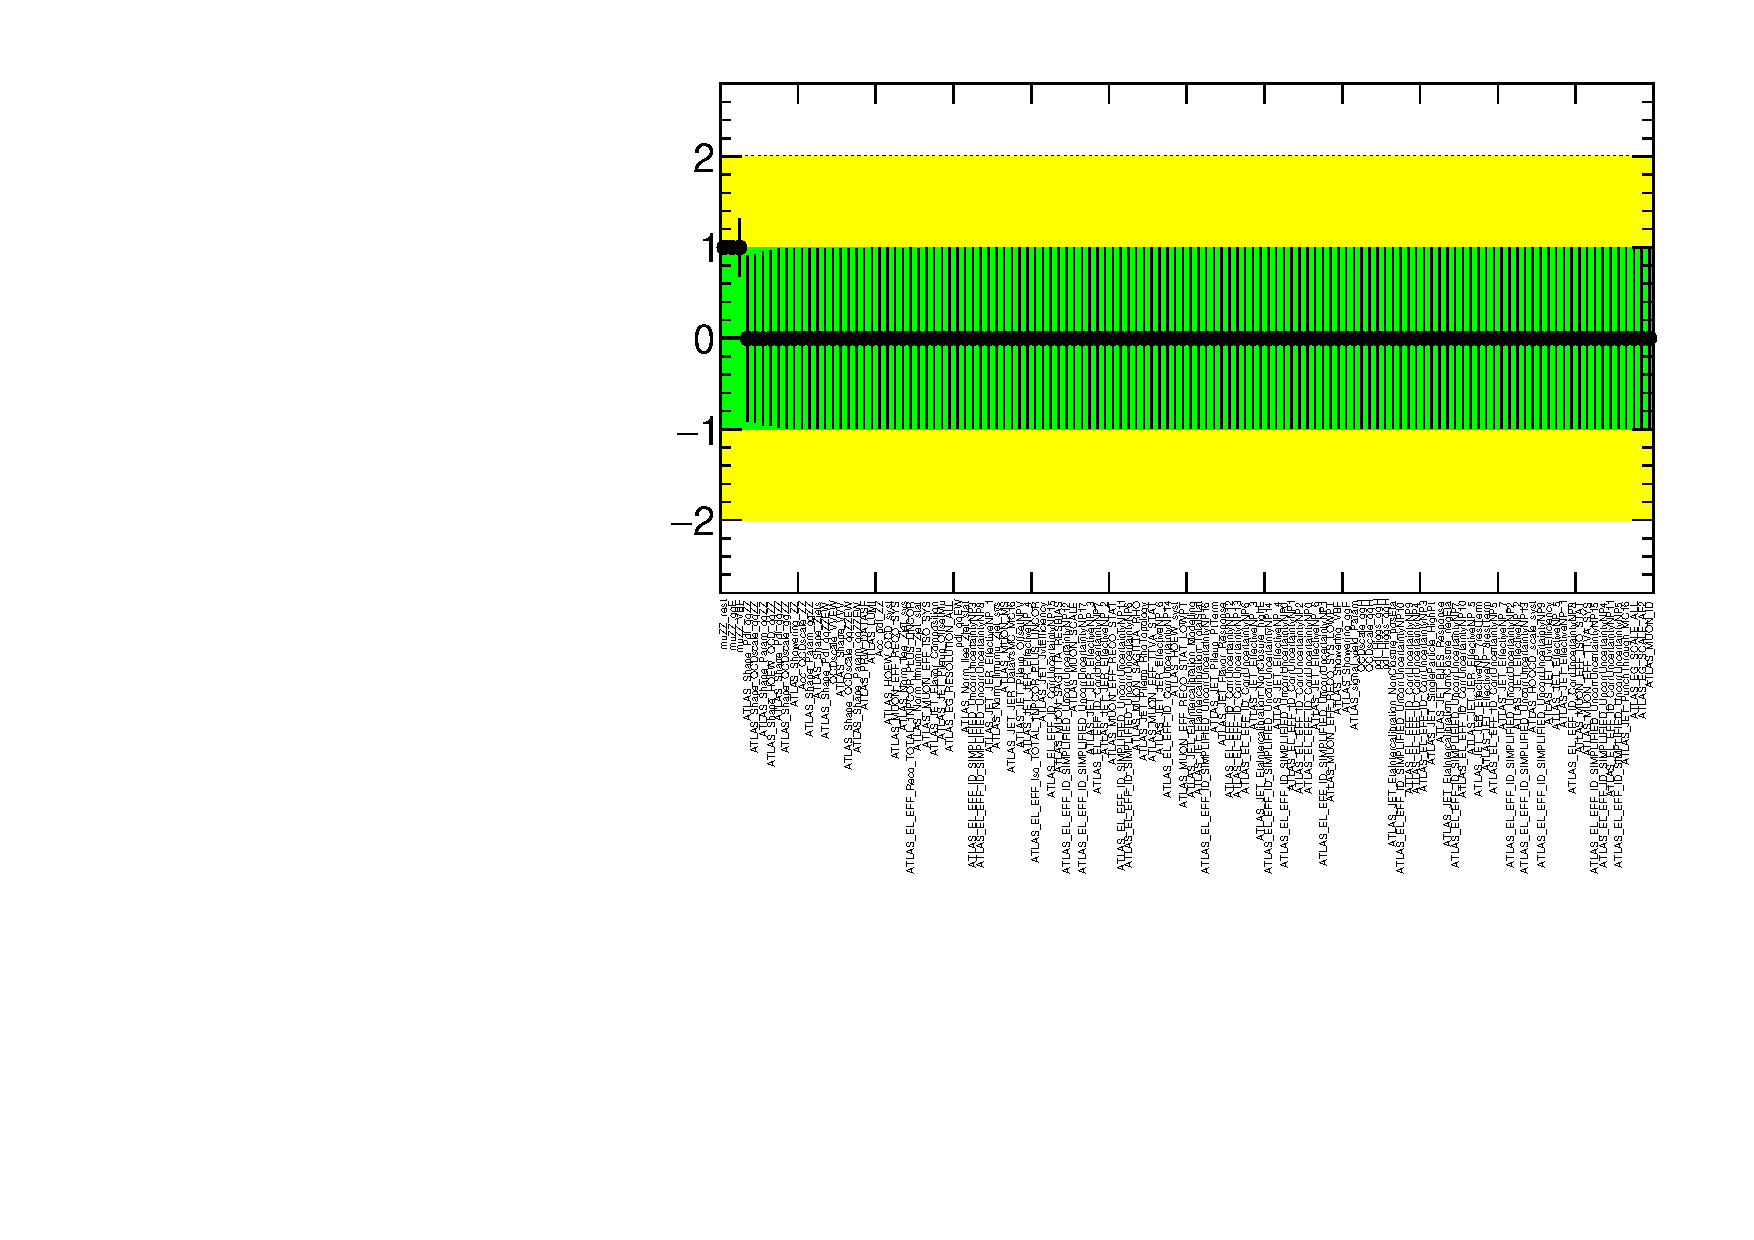
\includegraphics[width=0.8\figwidth]{figures/HMHZZ/results/Pulls_NWA_floatZZ_dnn_Asimov.pdf}}\\
\subfloat[]{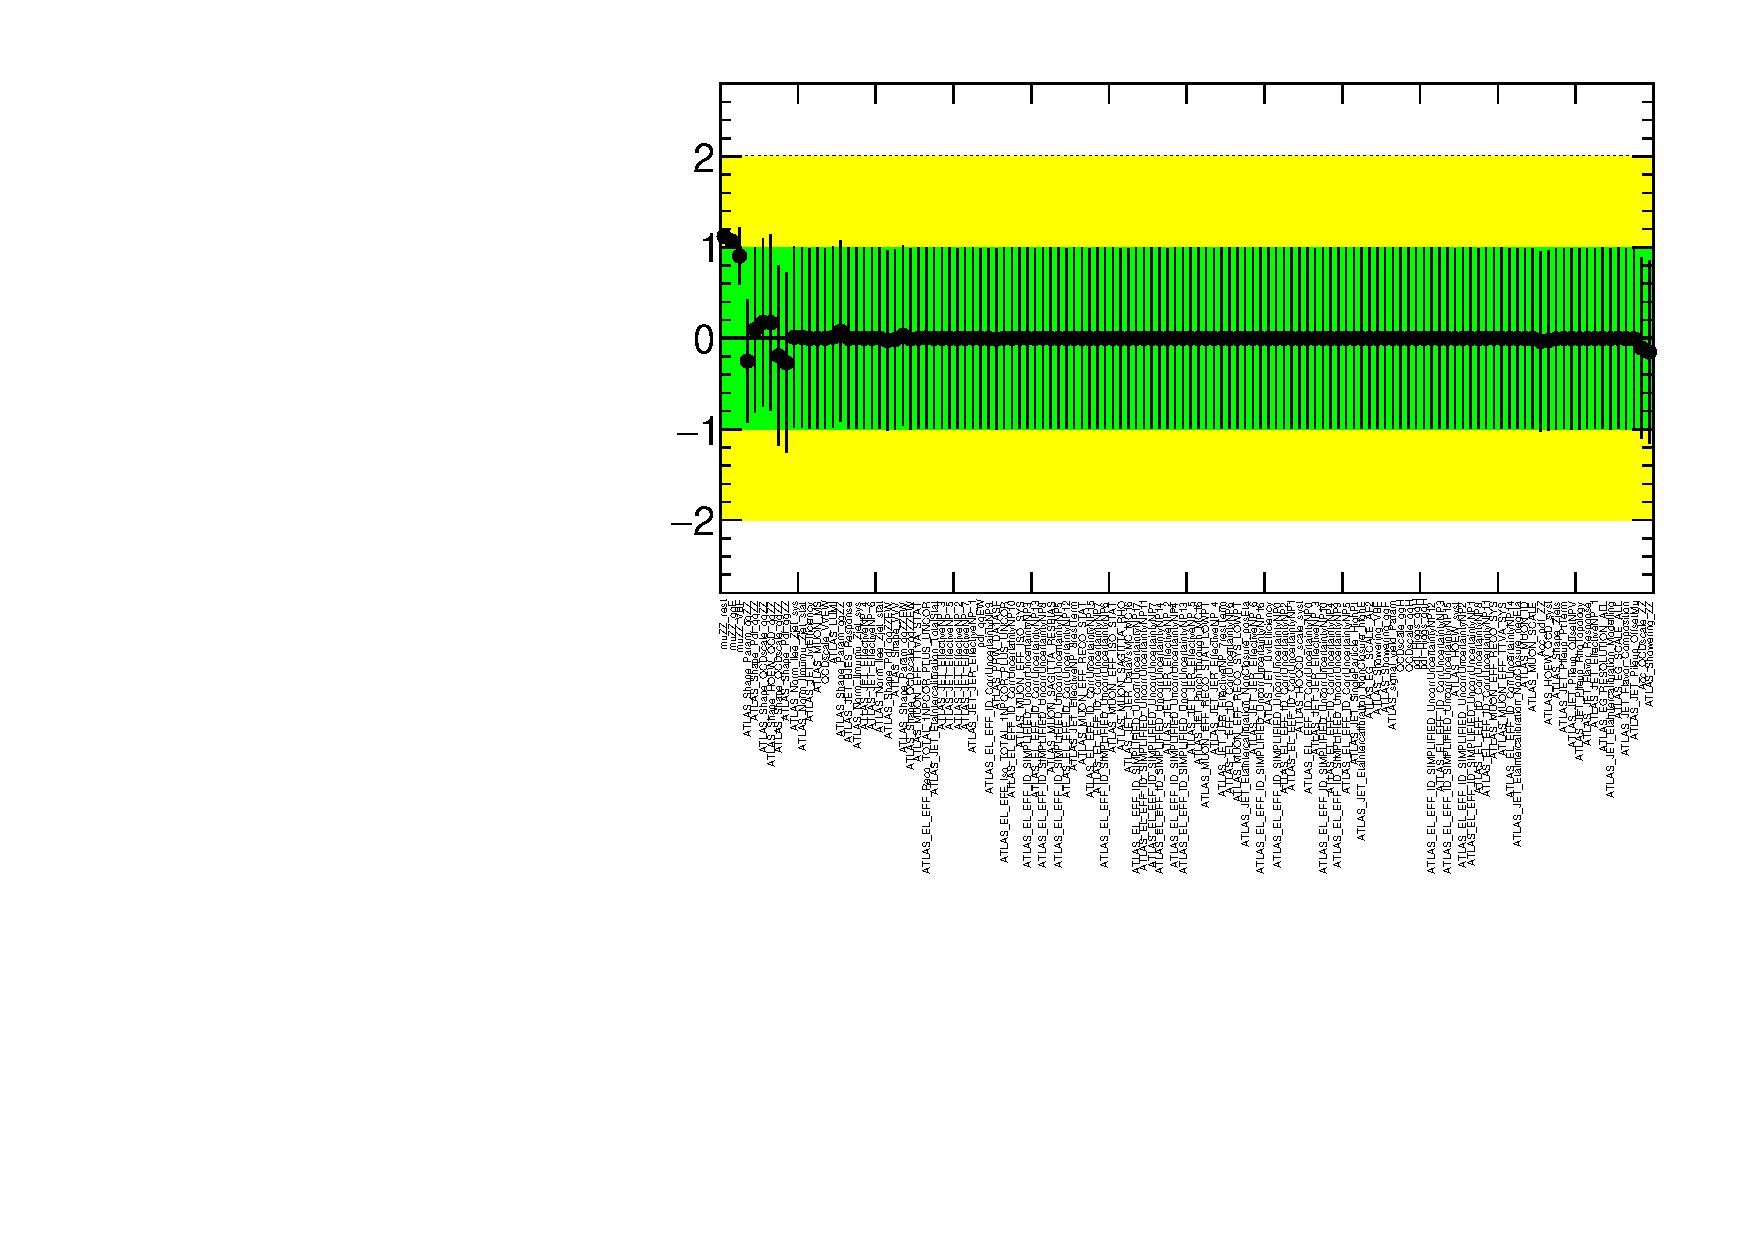
\includegraphics[width=0.8\figwidth]{figures/HMHZZ/results/Pulls_NWA_floatZZ_dnn_Obs.pdf}}
\caption{Pulls and constraints of nuisance parameters after a background only fit to (a) Asimov data and (b) observed data in the \llll channel.
The Asimov data is generated with background data only, and the observed data includes datasets from 2015 to 2018.
}
\label{fig:NPpull_cb_asimov}
\end{center}
\end{figure}

\begin{figure}[!ht]
\begin{center}
\subfloat[]{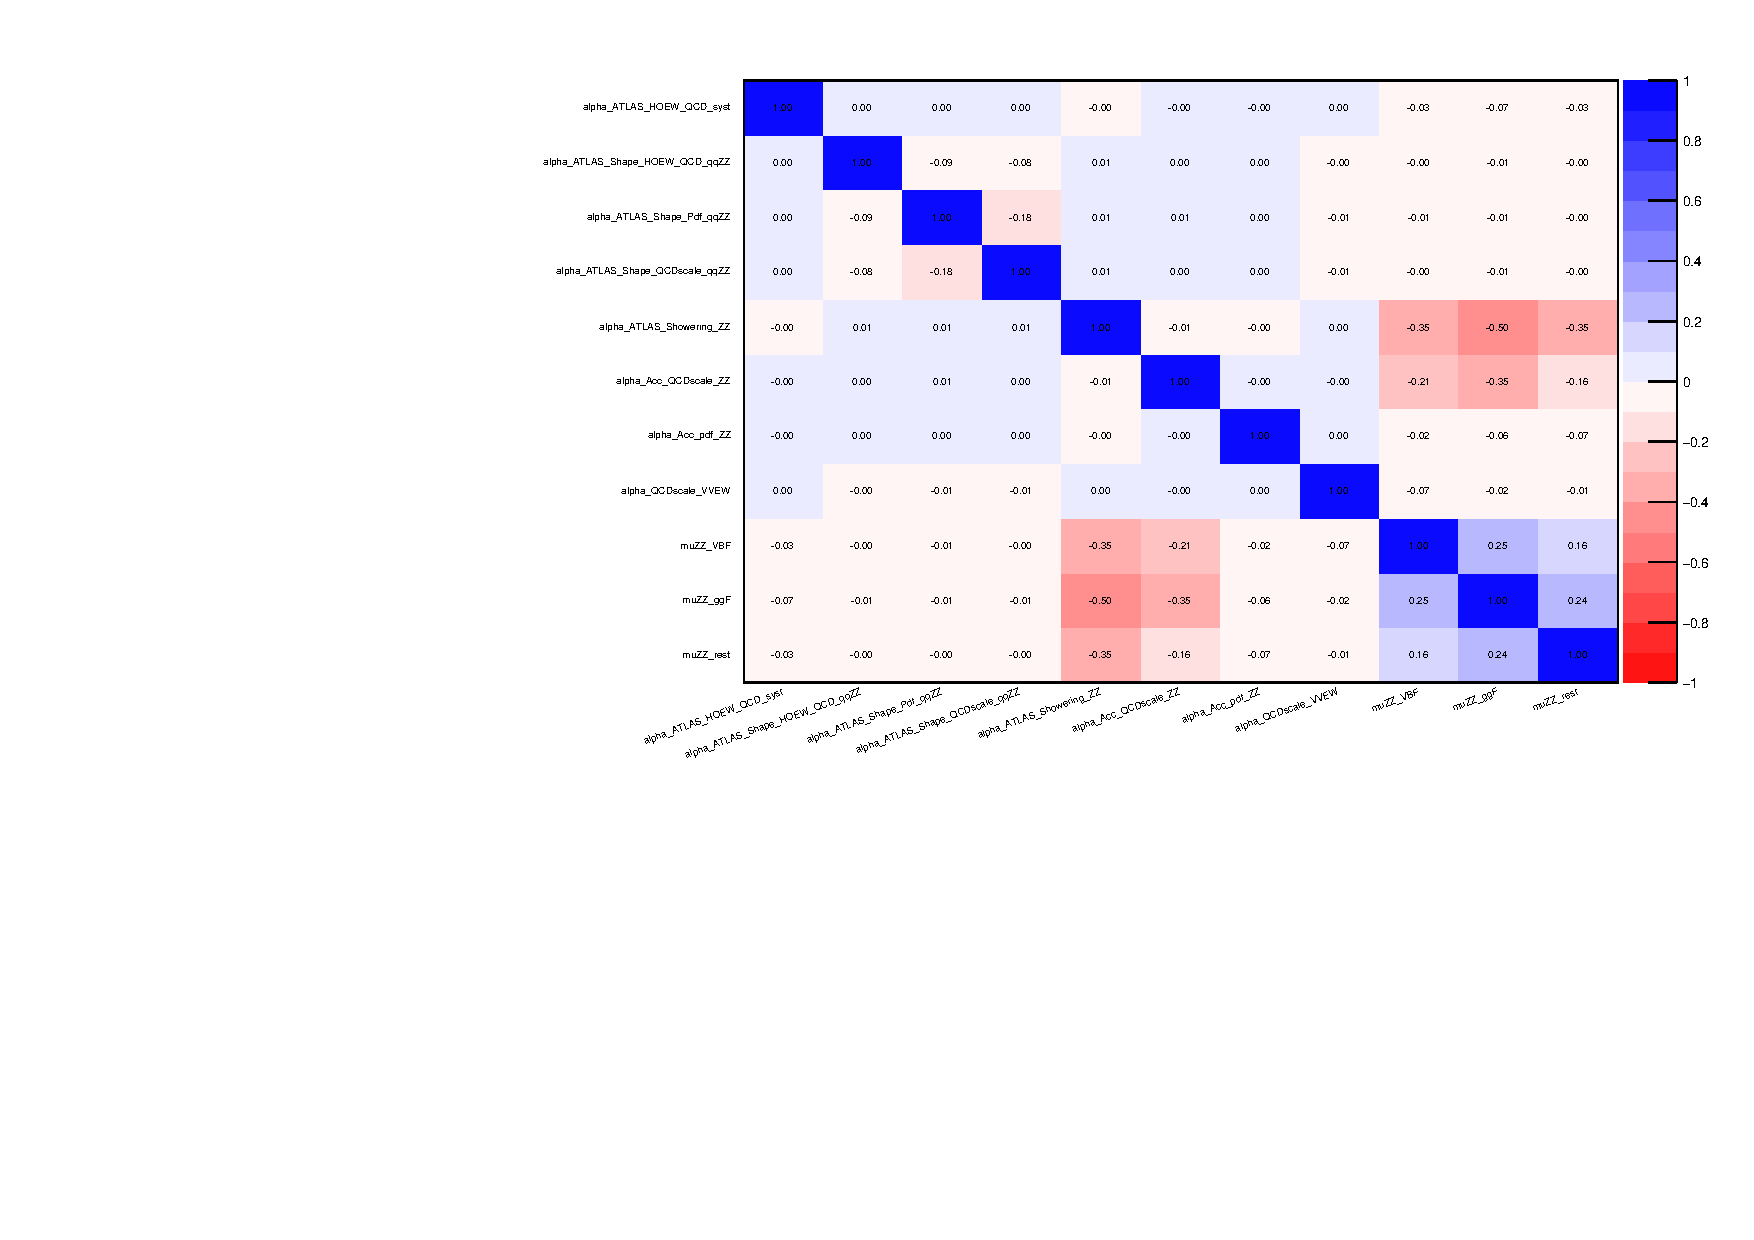
\includegraphics[width=0.8\figwidth]{figures/HMHZZ/results/Correlation_NWA_floatZZ_dnn_Asimov.pdf}}
\caption{Correlation of nuisance parameters after a background only fit to Asimov data in the \llll channel.
The Asimov data is generated with background data only.
}
\label{fig:NPcorr_cb_asimov}
\end{center}
\end{figure}

The impact of a systematic uncertainty on the result depends on the production mode as well as the mass hypothesis.
To check the impact of systematic uncertainties on expected signal sensitivity, a NP ranking study is performed using
signal injected Asimov data with the injected cross section close to 95\% CLs upper limit at two masses: 400~\gev and 1000~\gev.
The results are shown in Fig.~\ref{fig:rank_cb_NWA_ggF} (\ref{fig:rank_cb_NWA_VBF}) for ggF (VBF) production mode.
For ggF production, at lower masses, the systematic uncertainties of parton showering variation for signal, the luminosity uncertainty, and the and the parametrization of signal acceptance
dominate,
while at higher masses, the shape uncertainties from PDF variation for ZZ (\qqZZ and \ggZZ) background become important, as also seen in VBF production mode.
For VBF production, jet related uncertainties become more important comparing to ggF production.
In addition, the dominate uncertainties include the acceptance uncertainty from QCD scale variation for signal and the luminosity uncertainty.

\begin{figure}[!ht]
\begin{center}
\subfloat[]{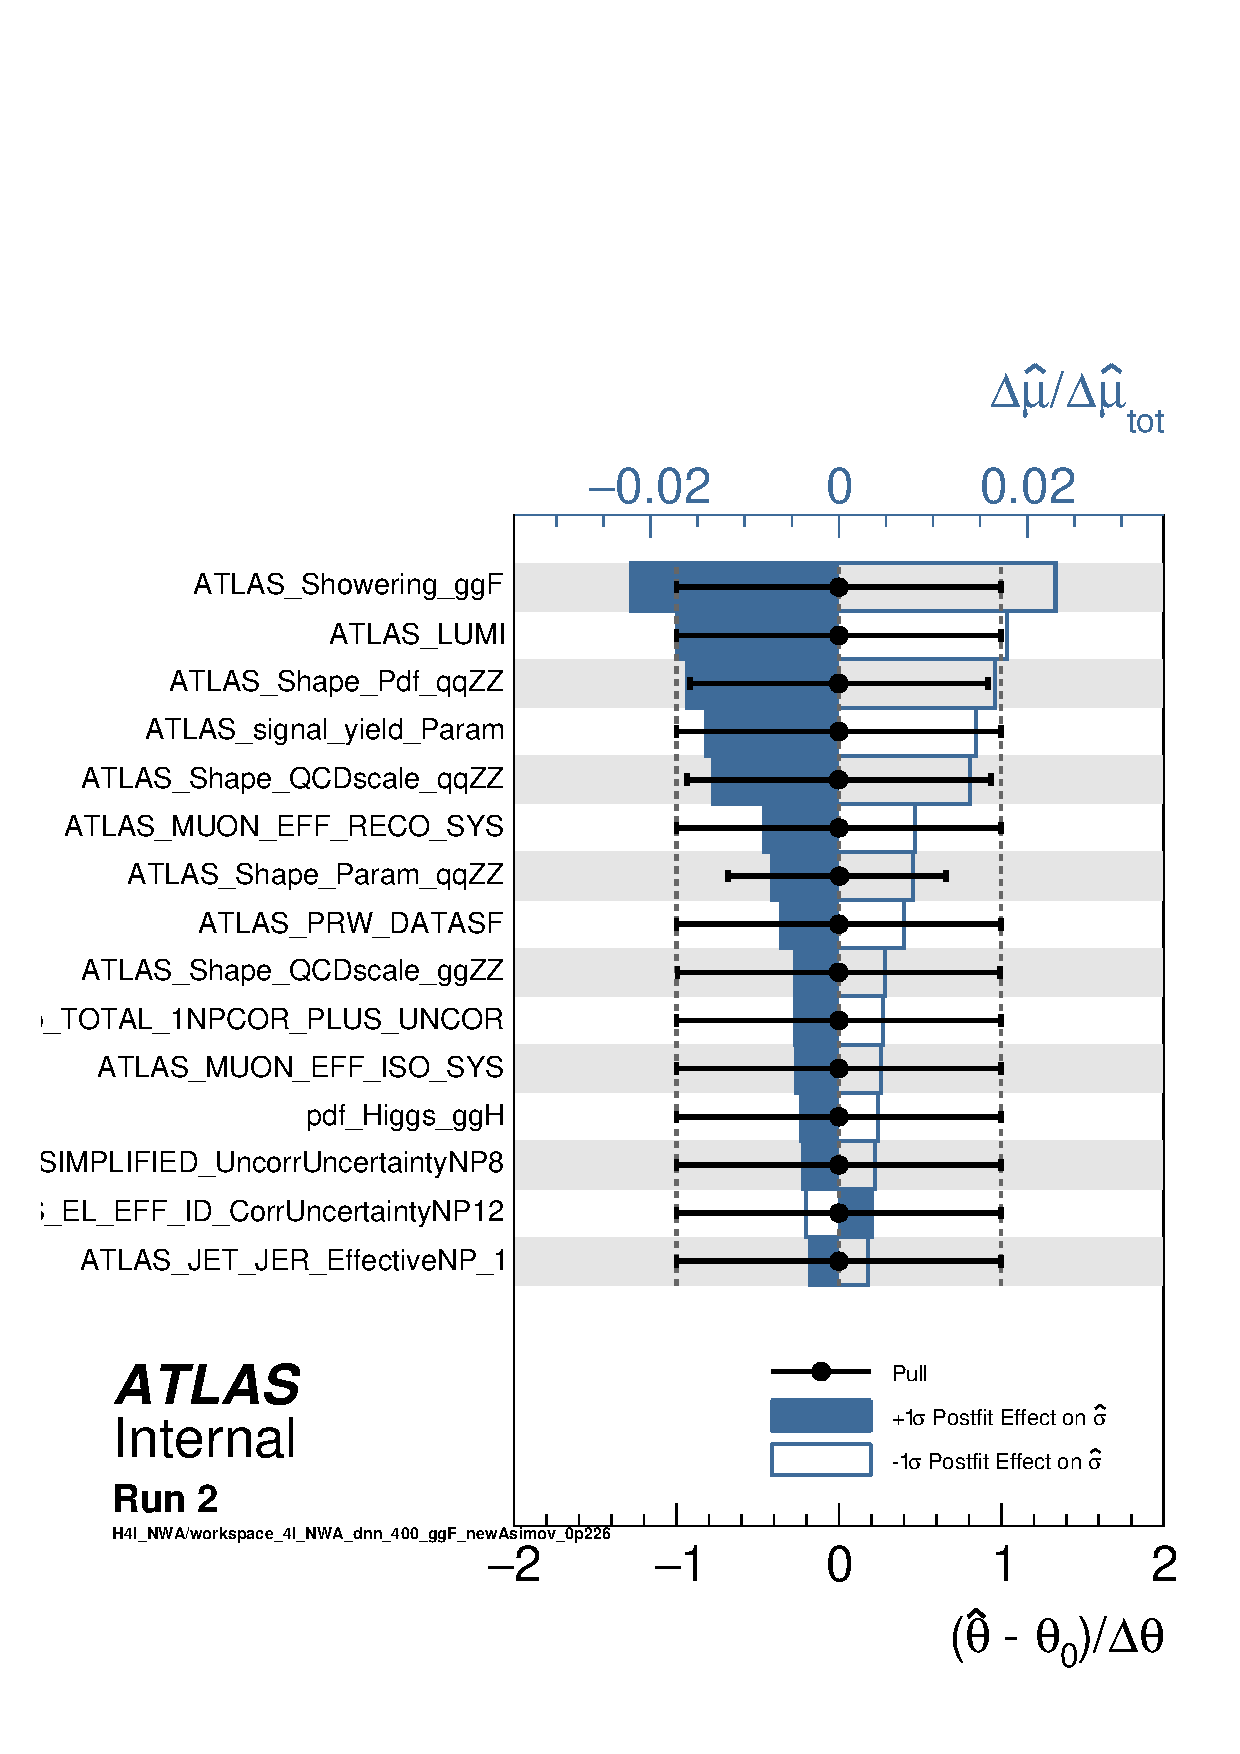
\includegraphics[width=0.48\figwidth]{figures/HMHZZ/results/workspace_4l_NWA_dnn_400_ggF_newAsimov_0p226_pulls_paper.pdf}}
\subfloat[]{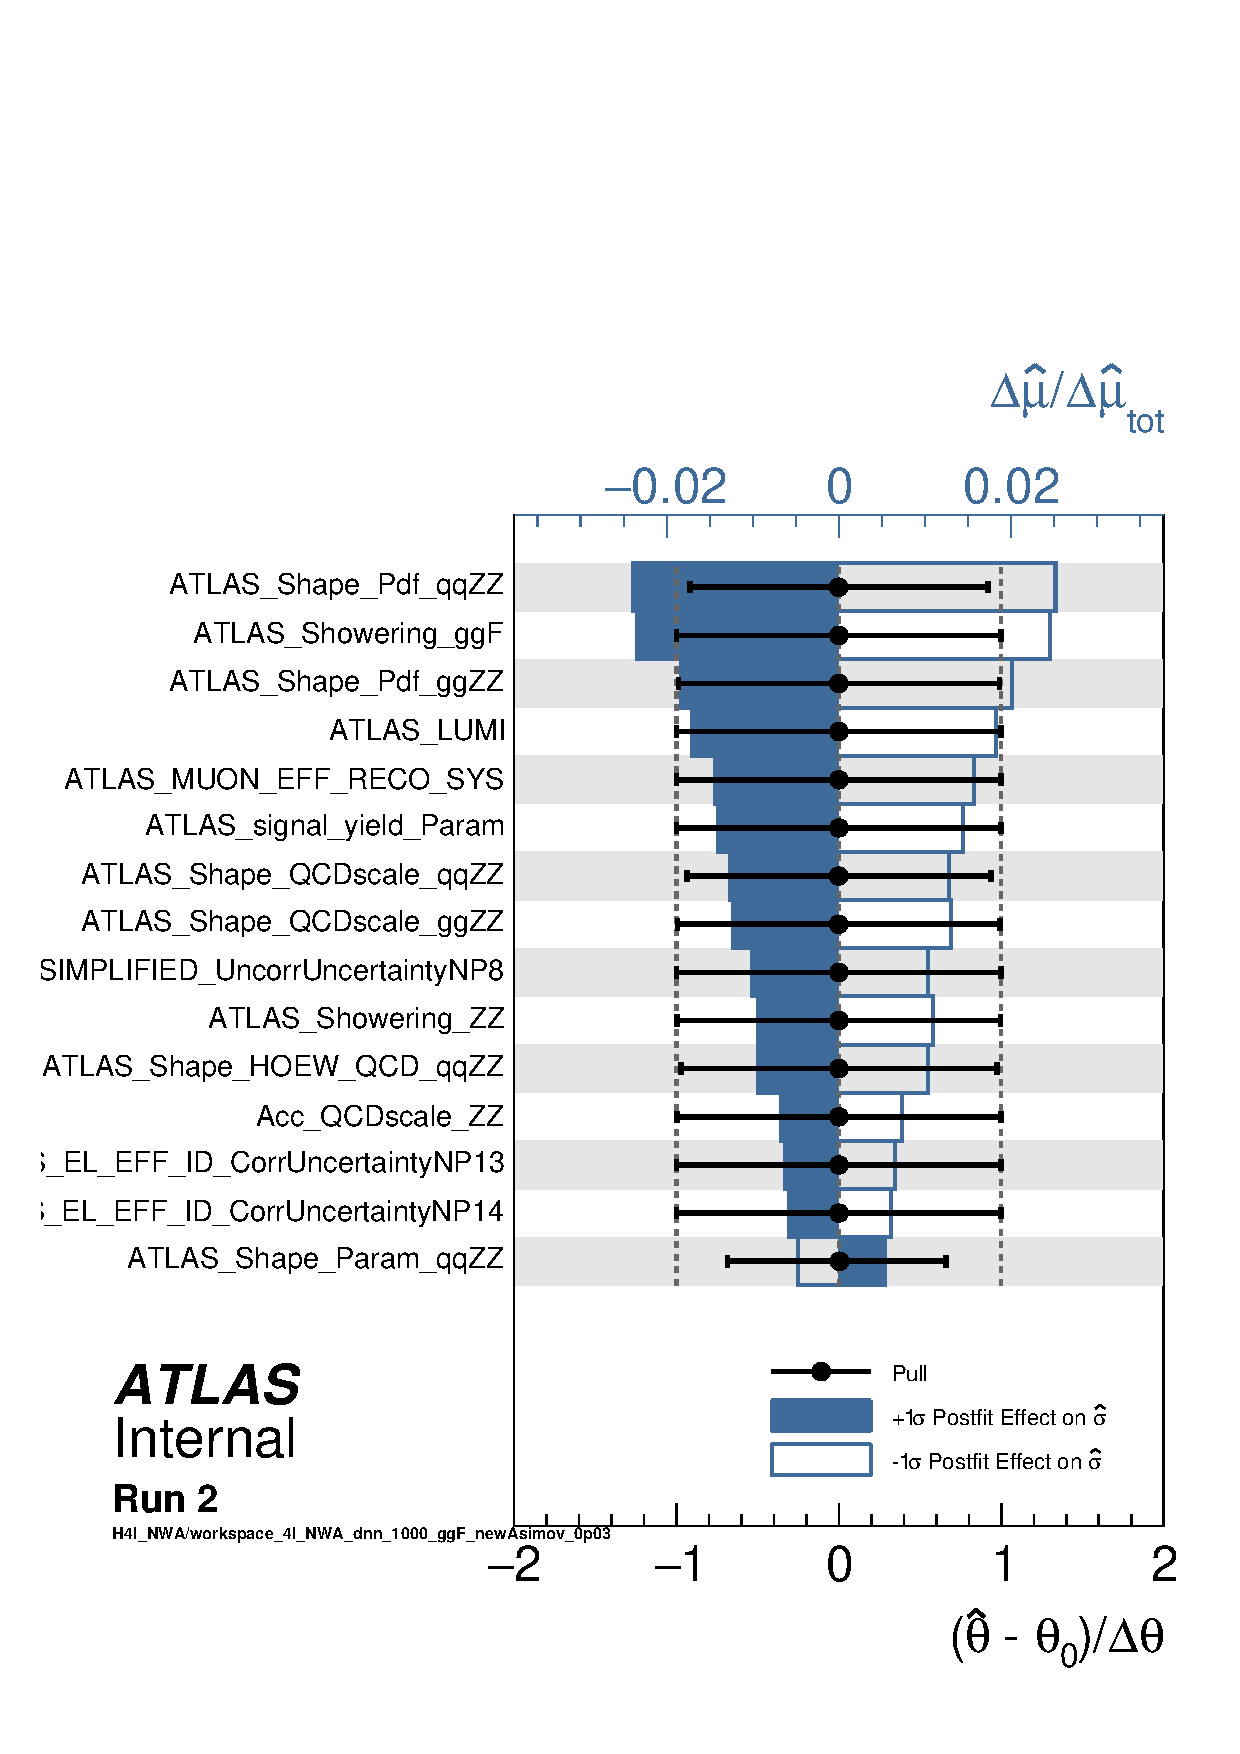
\includegraphics[width=0.48\figwidth]{figures/HMHZZ/results/workspace_4l_NWA_dnn_1000_ggF_newAsimov_0p03_pulls_paper.pdf}}
\caption{NP ranking plot for the \xsggF\ fit to Asimov data in the \llll channel.
The Asimov data is injected with \xsggF\ = 0.226 fb for $m_H = 400$ GeV (left) and \xsggF\ = 0.030 fb for $m_H = 1000$ GeV (right).
}
\label{fig:rank_cb_NWA_ggF}
\end{center}
\end{figure}

\begin{figure}[!ht]
\begin{center}
\subfloat[]{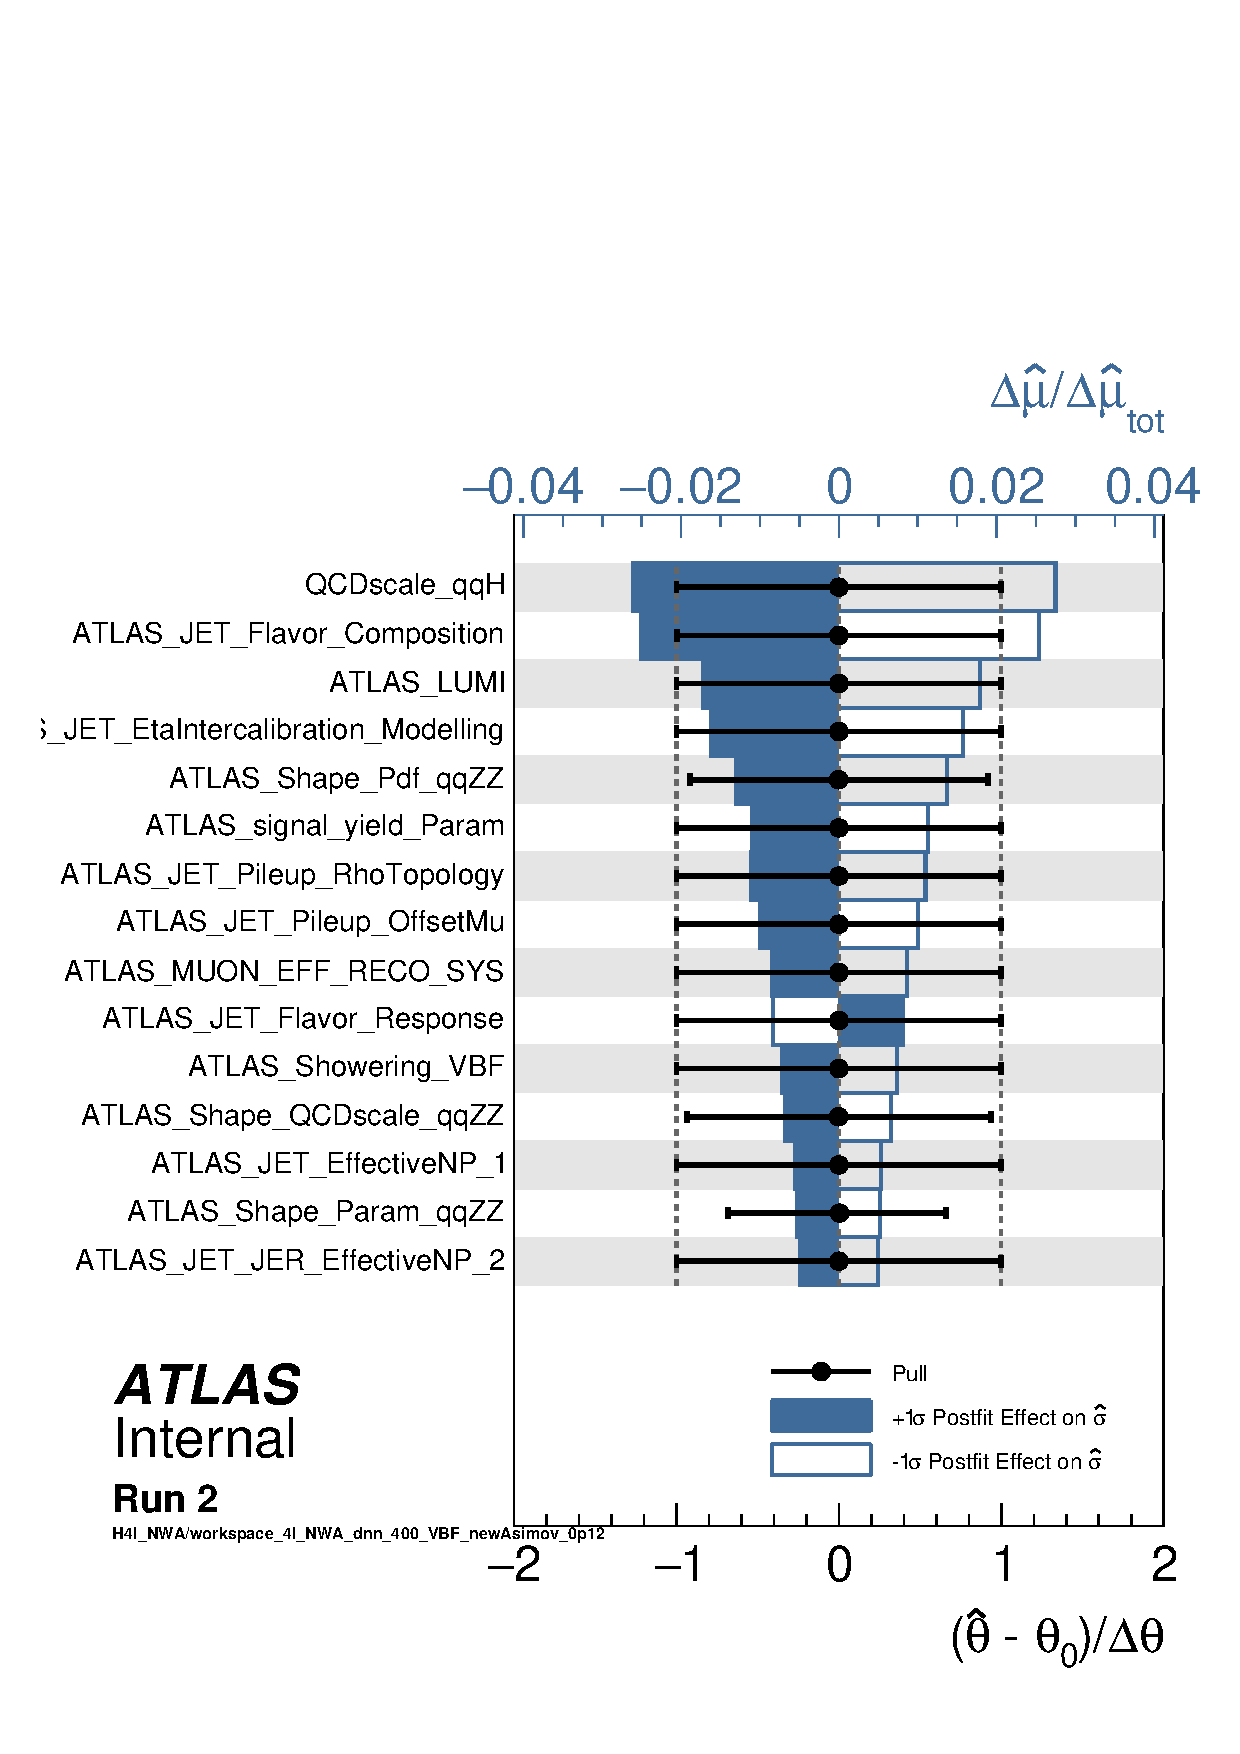
\includegraphics[width=0.48\figwidth]{figures/HMHZZ/results/workspace_4l_NWA_dnn_400_VBF_newAsimov_0p12_pulls_paper.pdf}}
\subfloat[]{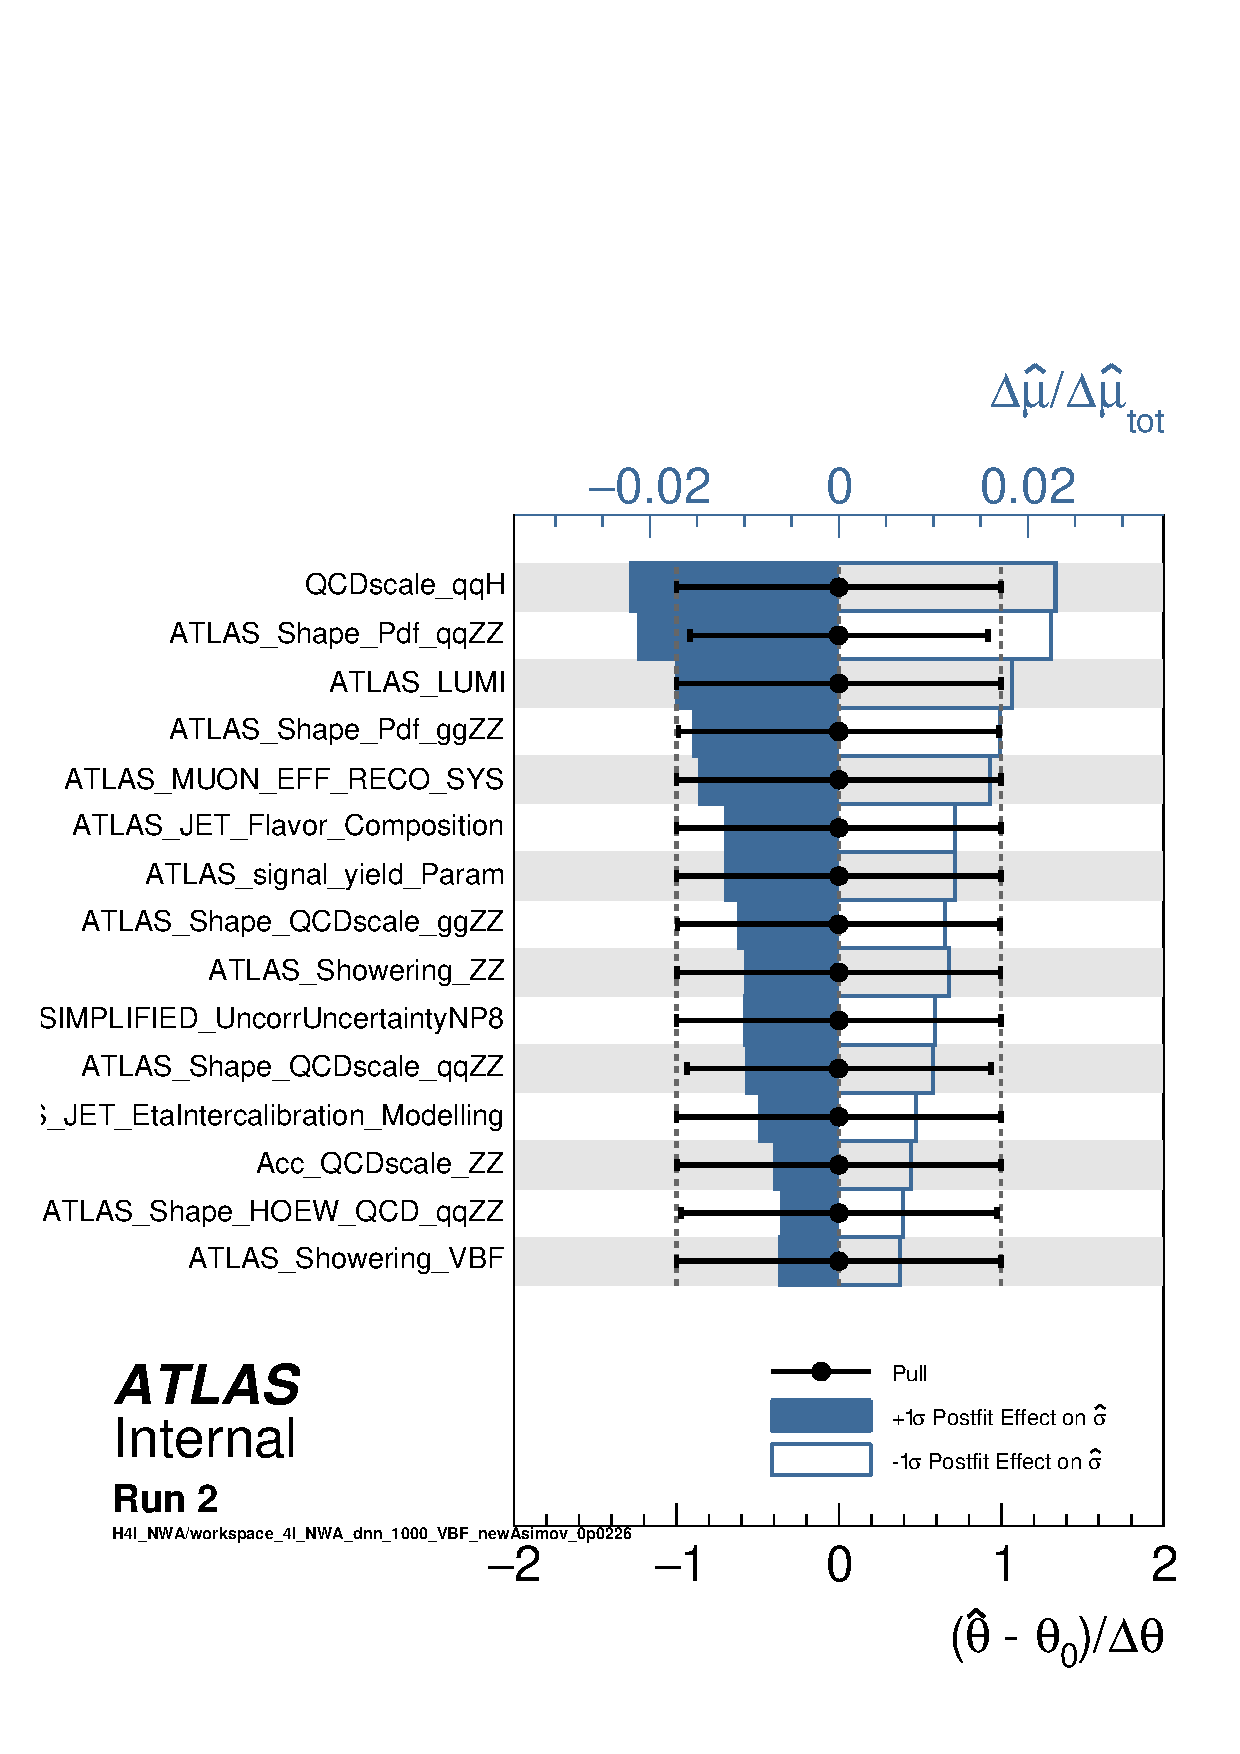
\includegraphics[width=0.48\figwidth]{figures/HMHZZ/results/workspace_4l_NWA_dnn_1000_VBF_newAsimov_0p0226_pulls_paper.pdf}}
\caption{NP ranking plot for the \xsVBF\ fit to Asimov data in the \llll channel.
The Asimov data is injected with \xsVBF\ = 0.120 fb for $m_H = 400$ GeV (left) and \xsVBF\ = 0.0226 fb for $m_H = 1000$ GeV (right).
}
\label{fig:rank_cb_NWA_VBF}
\end{center}
\end{figure}


%% =======================================================================================================
\subsection{Interpretations}

\subsubsection{Spin-0 resonance with NWA}

In the absence of a specific model, the ratio of ggF and VBF production mode is unknown for this additional heavy scalar.
For this reason, the fits for ggF and VBF processes are done separately, and in each case the cross section of the other process is allow to be a free parameter in fit.
The observed and expected upper limit at 95\% confidence level (CL) on the $\sigma \times BR(H \rightarrow ZZ)$ of a narrow scalar resonance for both ggF (left) and VBF (right) production mode with the integrated luminosity of \lumi is shown in figure~\ref{fig:NWA201518_DNN} (\ref{fig:NWA201518_Cut}) for DNN- (cut-) based analysis.
No excess over 2$\sigma$ is found.

\begin{figure}[h]
    \centering
    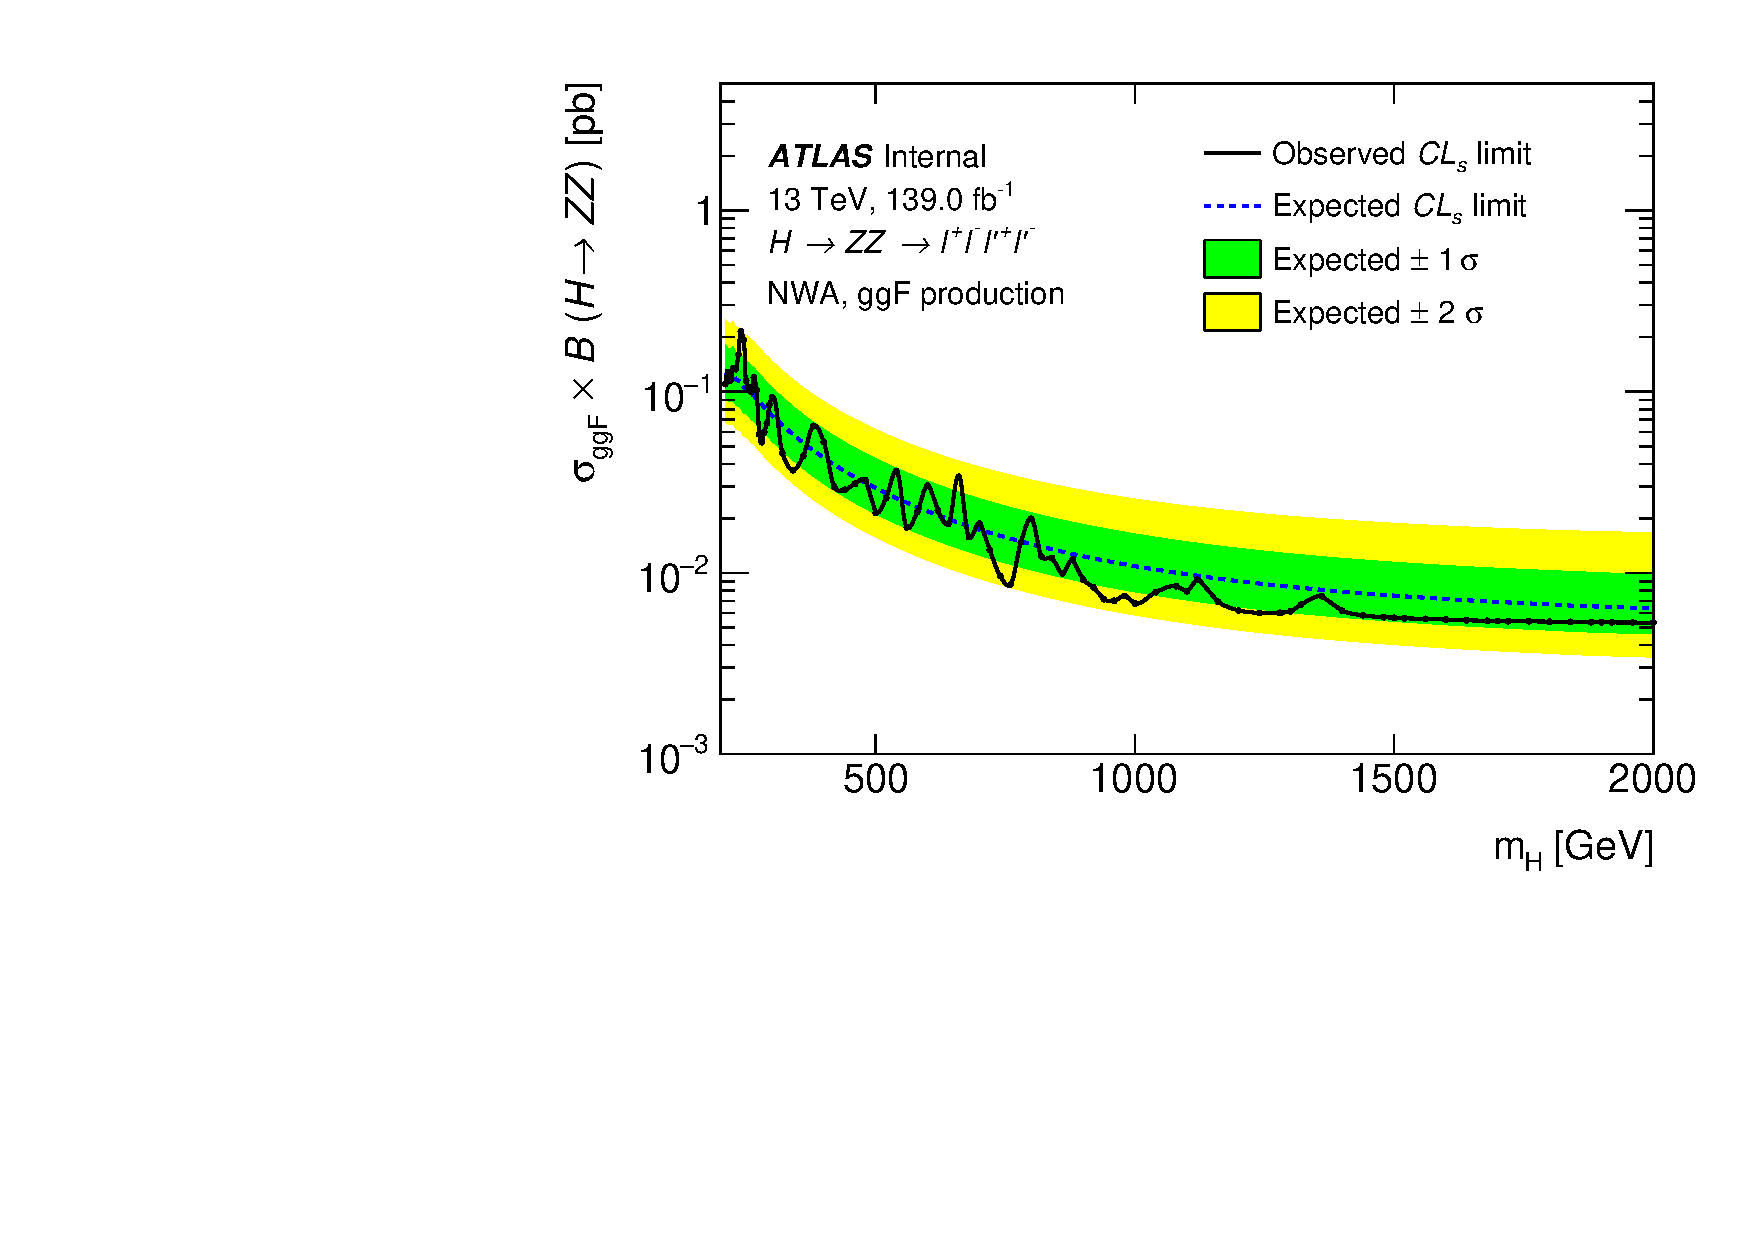
\includegraphics[width=0.48\textwidth]{figures/HMHZZ/results/limits_DNN_ggF.pdf}
    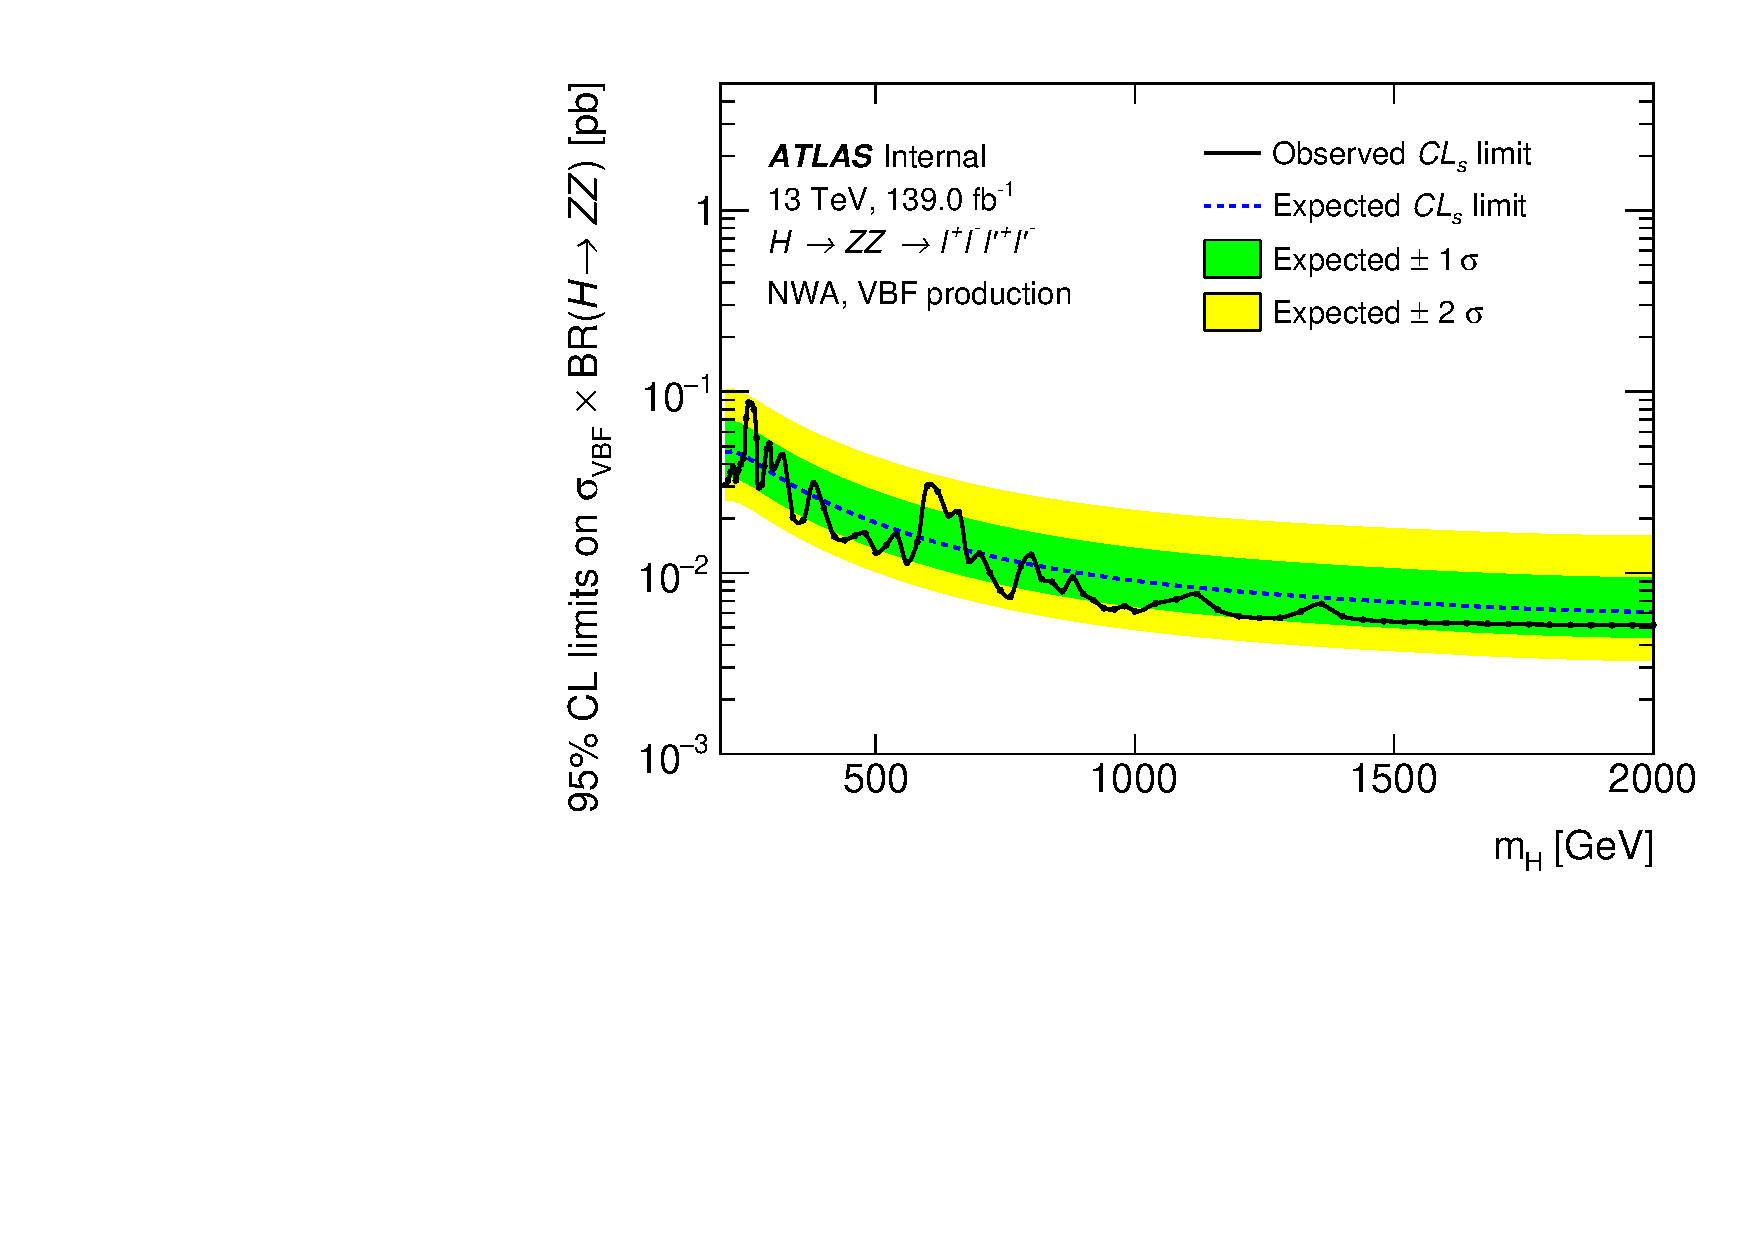
\includegraphics[width=0.48\textwidth]{figures/HMHZZ/results/limits_DNN_VBF.pdf}
    \caption{The expected and observed upper limits at 95\% CL on $\sigma \times BR(H \rightarrow ZZ)$ using the DNN-based analysis for ggF (left) and VBF (right) production. The green and yellow bands represent the $\pm 1\sigma$ and $\pm 2\sigma$ uncertainties in the expected limits.
 }
    \label{fig:NWA201518_DNN}
\end{figure}

\begin{figure}[h]
    \centering
    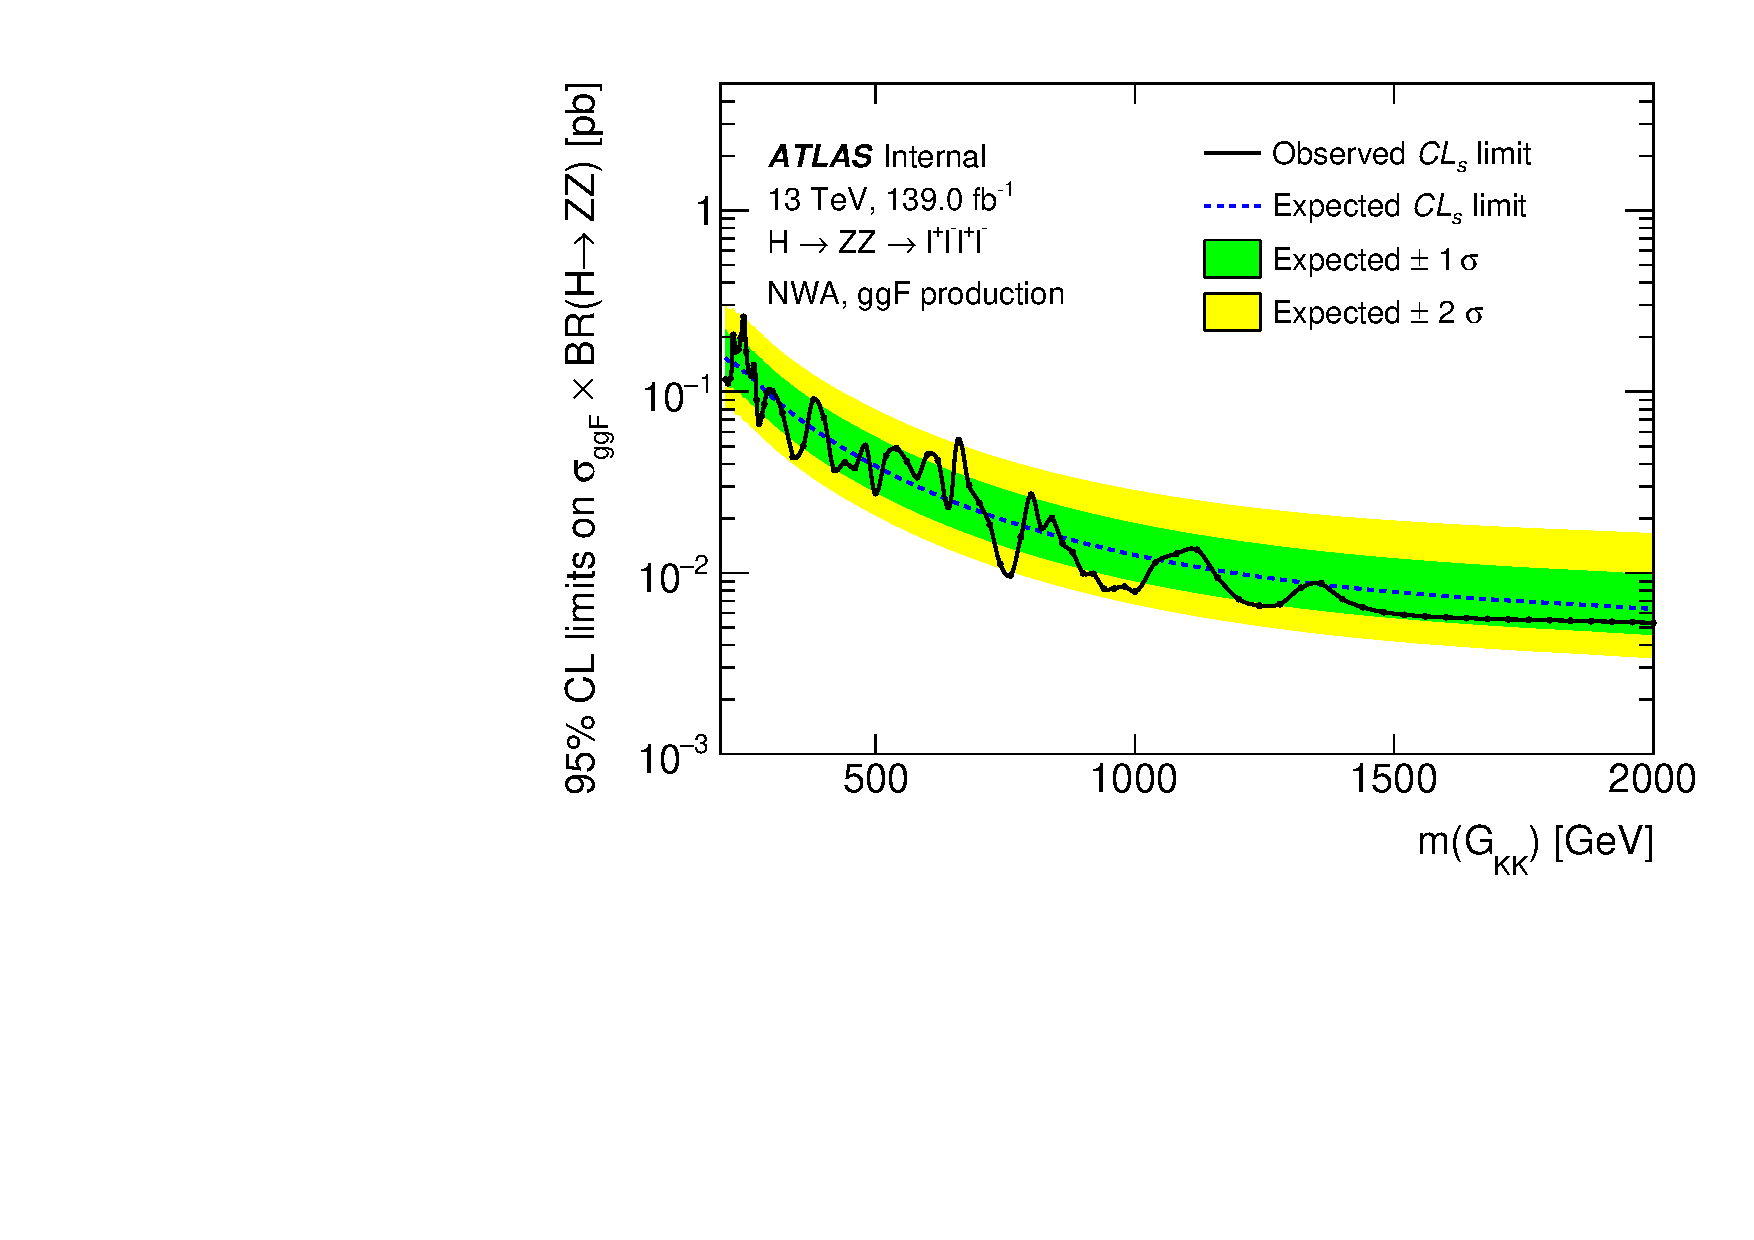
\includegraphics[width=0.48\textwidth]{figures/HMHZZ/results/limits_Cut2020_ggF.pdf}
    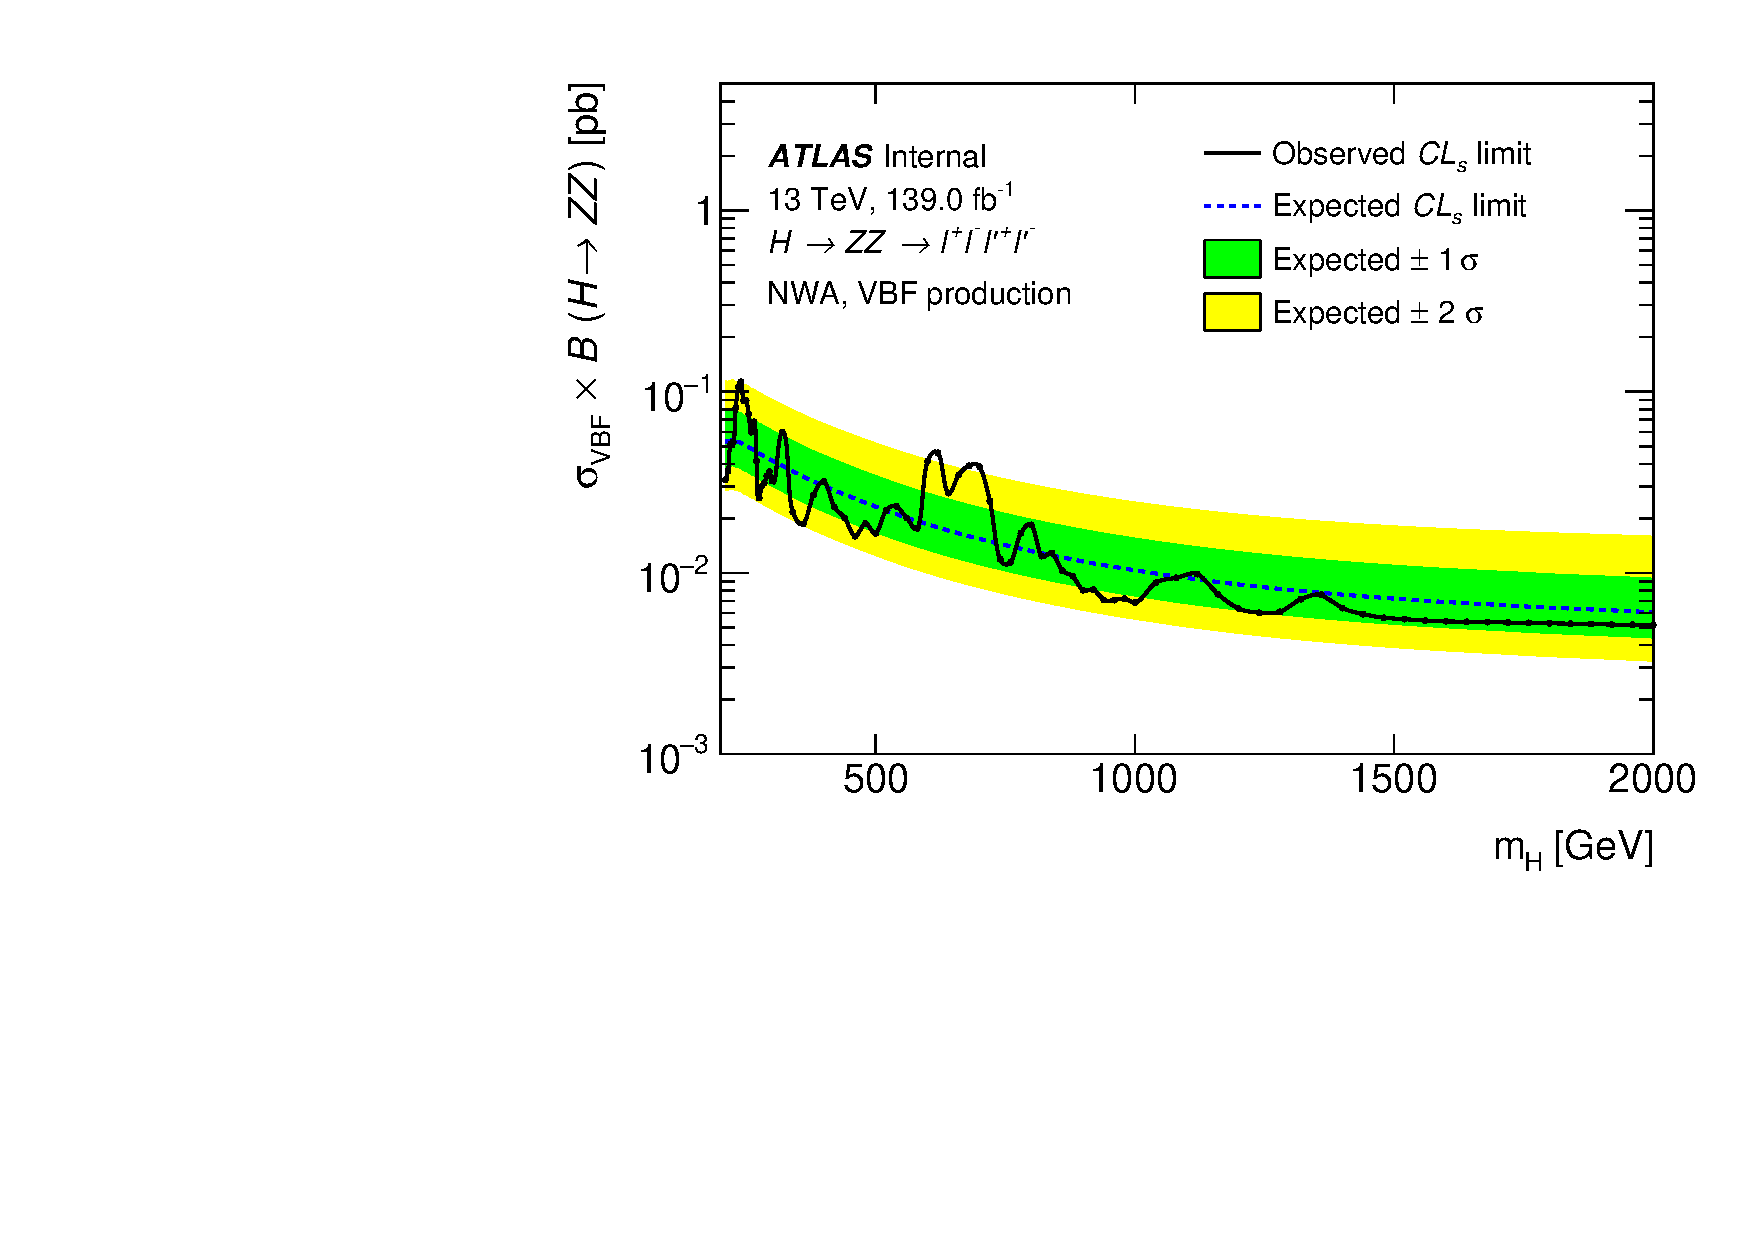
\includegraphics[width=0.48\textwidth]{figures/HMHZZ/results/limits_Cut2020_VBF.pdf}
    \caption{The expected and observed upper limits at 95\% CL on $\sigma \times BR(H \rightarrow ZZ)$ using the cut-based analysis for ggF (left) and VBF (right) production. The green and yellow bands represent the $\pm 1\sigma$ and $\pm 2\sigma$ uncertainties in the expected limits.
 }
    \label{fig:NWA201518_Cut}
\end{figure}

\subsubsection{Spin-0 resonance with LWA}

In the case of LWA model, only ggF production mode is studied.
The interference between the heavy scalar and SM Higgs boson (H-h), as well as the heavy scalar and SM \ggZZ continuum background (H-B) as modelled in section~\ref{sec:int_model} are considered.
The upper limit at 95\% confidence level (CL) on ggF cross section times branch ratio ($\sigma_{ggF} \times BR(H \rightarrow ZZ)$) is shown in figure~\ref{fig:LWAlimits_ggF_201518_withInt} for a width of 1\%, 5\%, 10\% and 15\% of \mH.

\begin{figure}[h]
    \begin{center}
    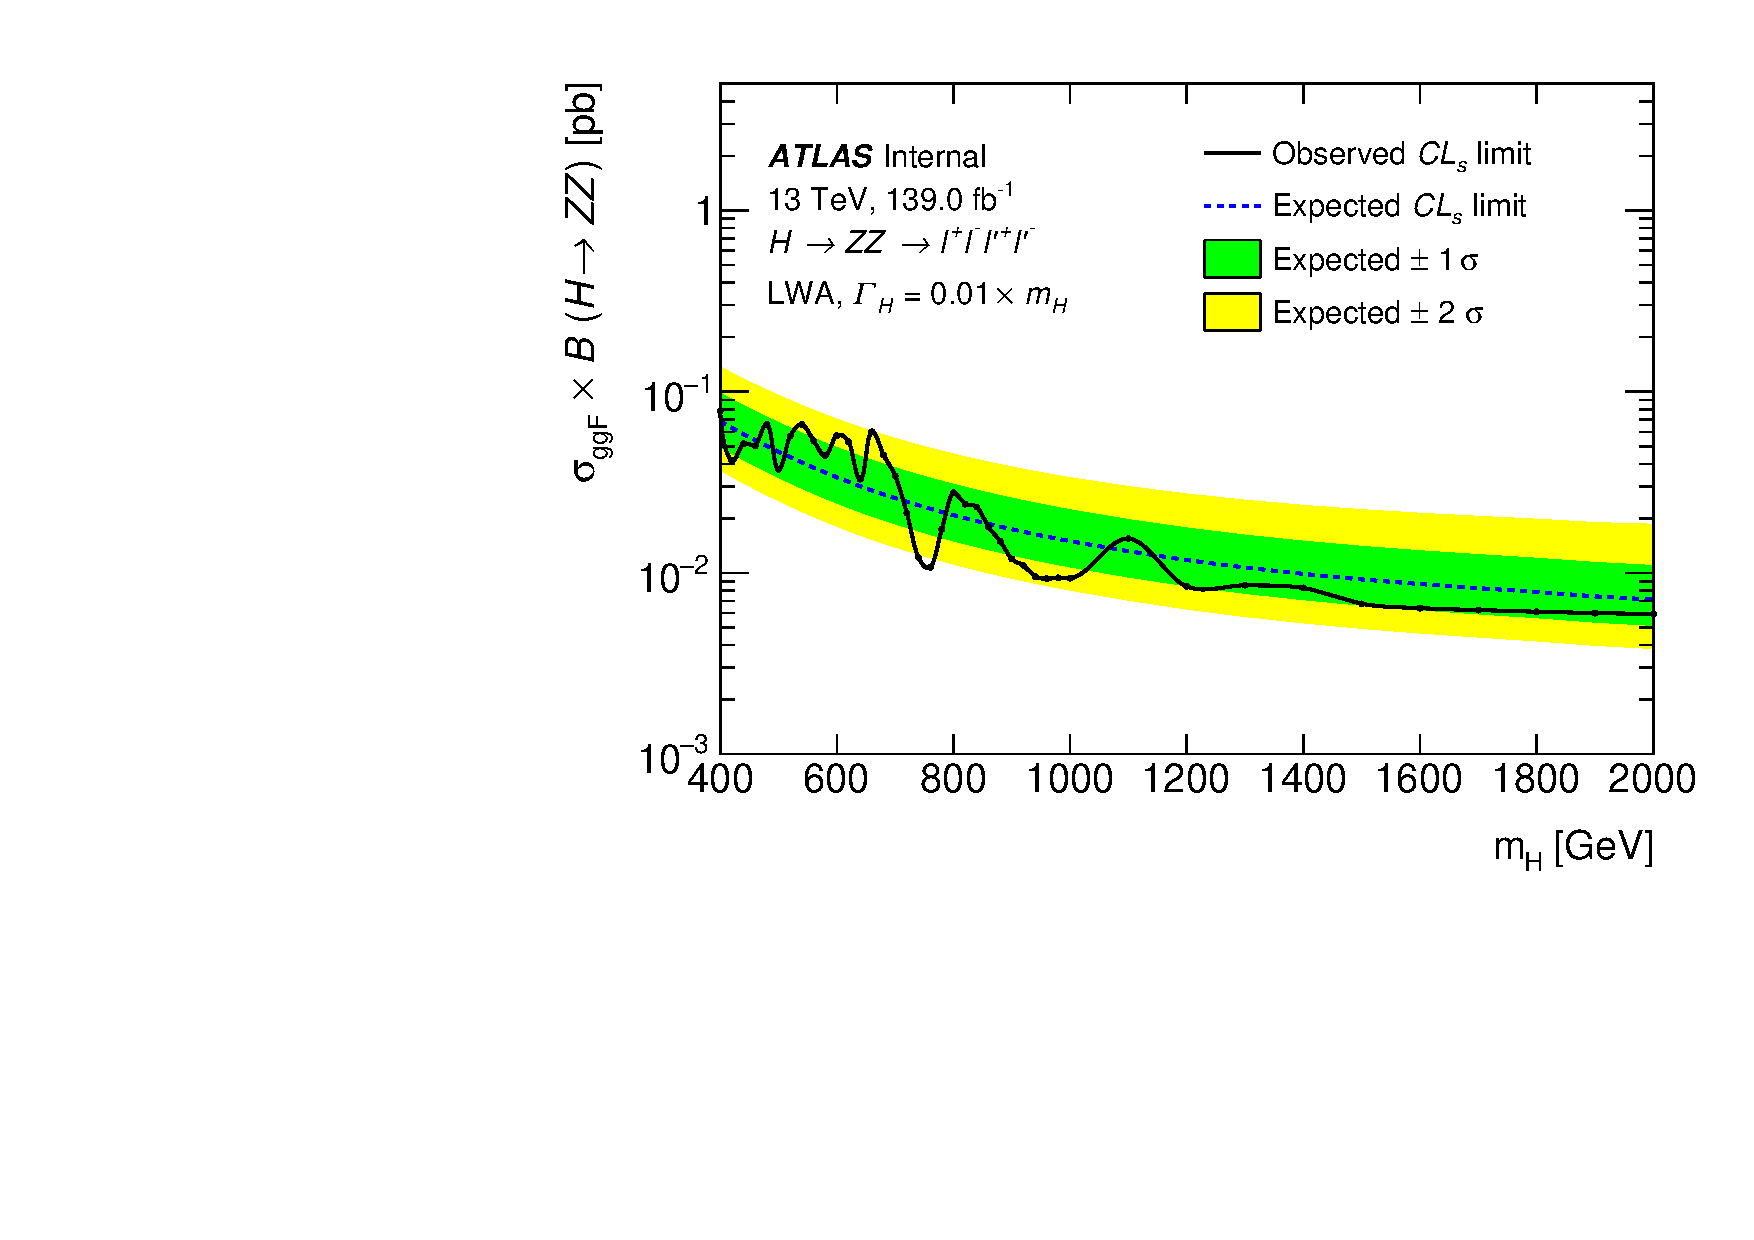
\includegraphics[width=0.48\textwidth]{figures/HMHZZ/results/Limits_LWA_withInt_1.pdf}
    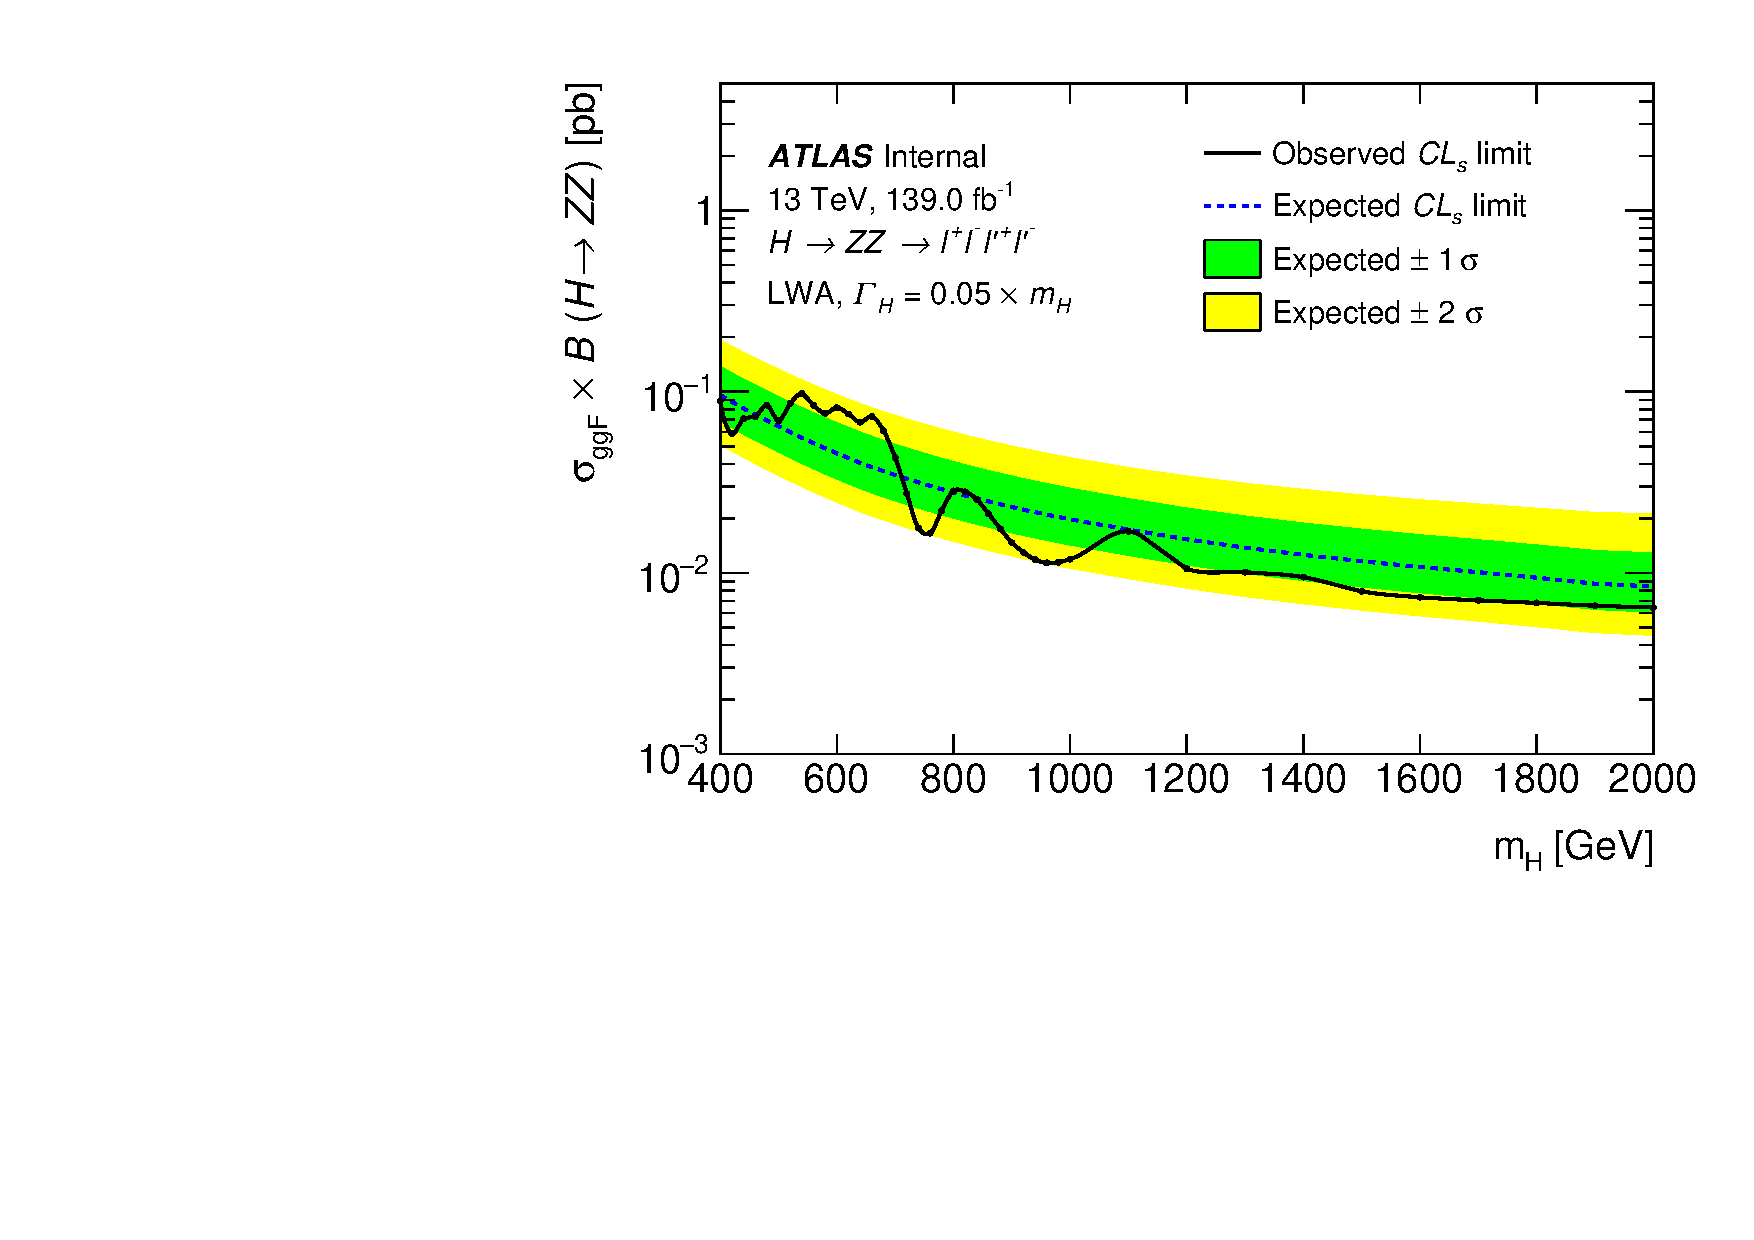
\includegraphics[width=0.48\textwidth]{figures/HMHZZ/results/Limits_LWA_withInt_5.pdf} \\
    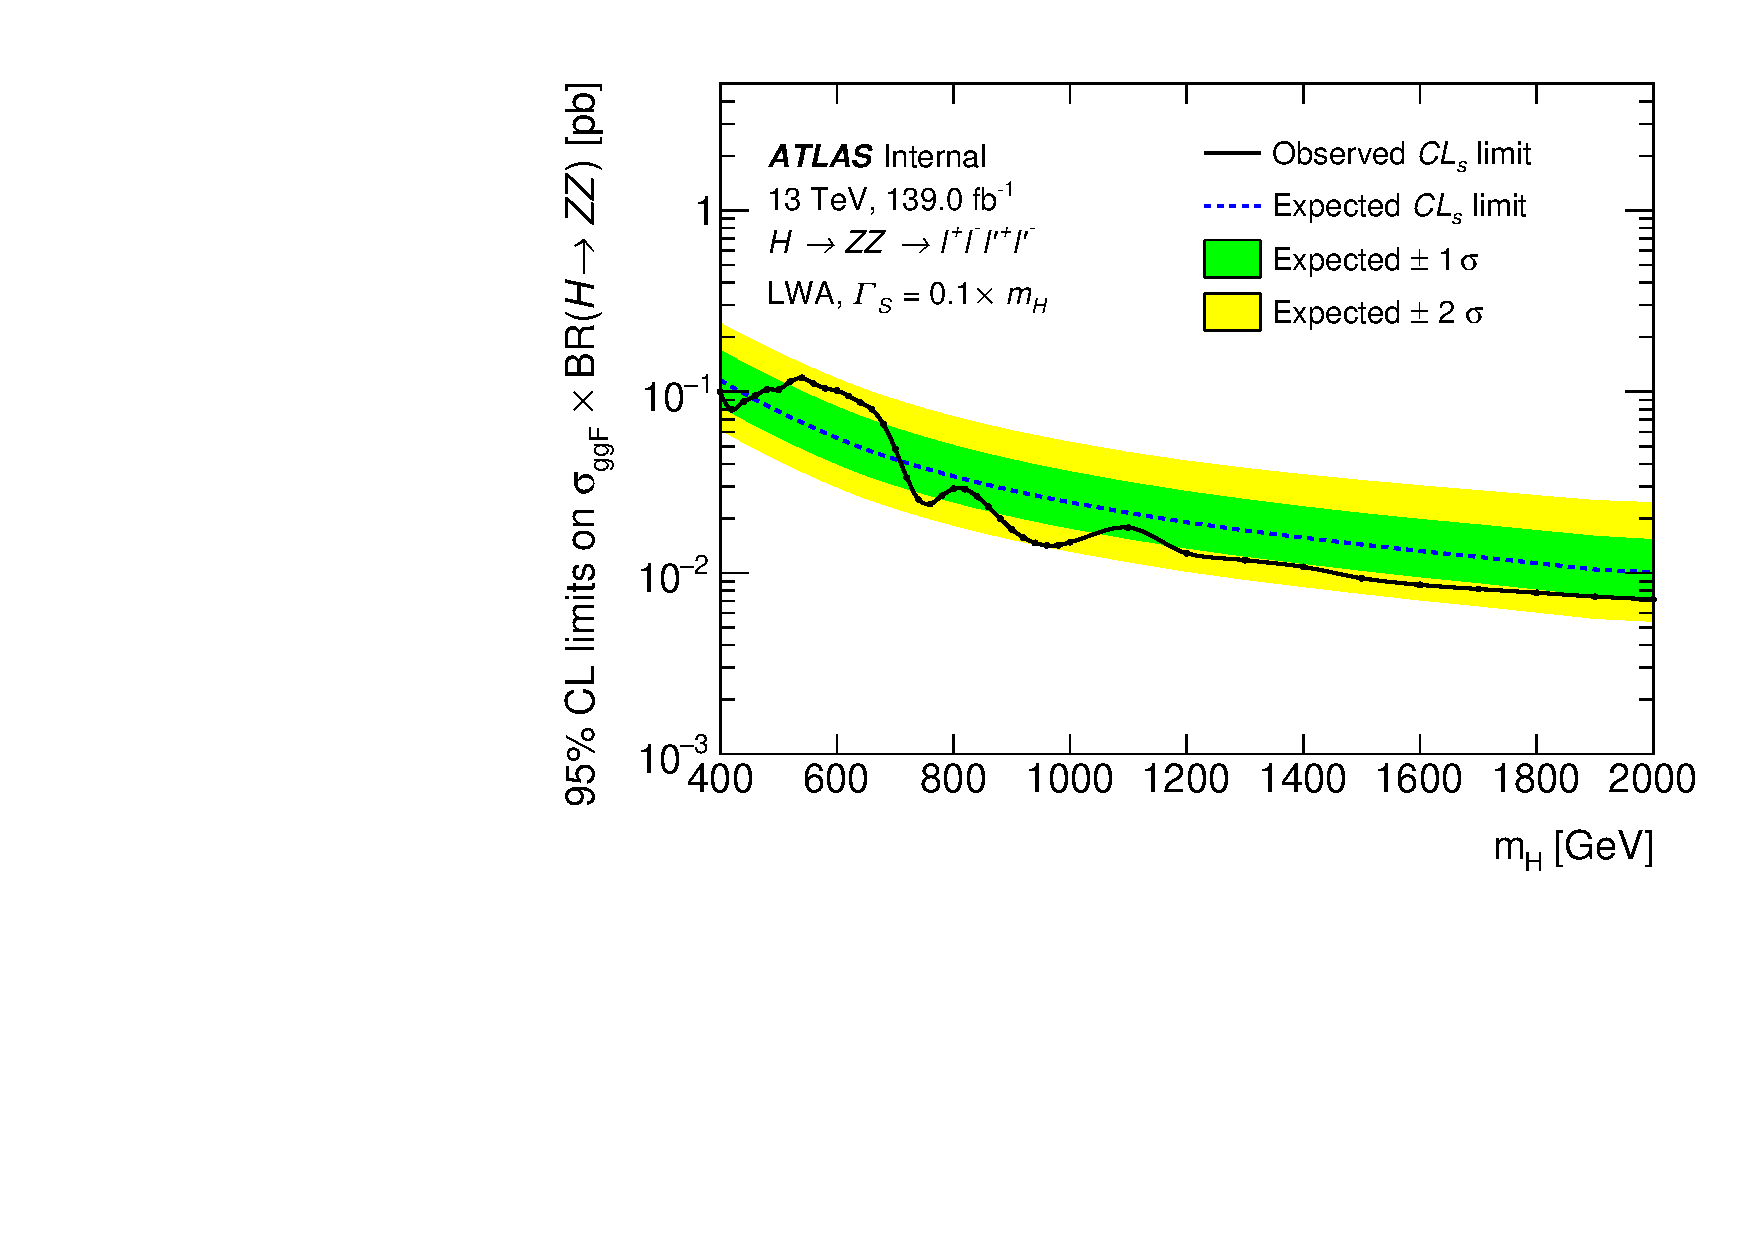
\includegraphics[width=0.48\textwidth]{figures/HMHZZ/results/Limits_LWA_withInt_10.pdf}
    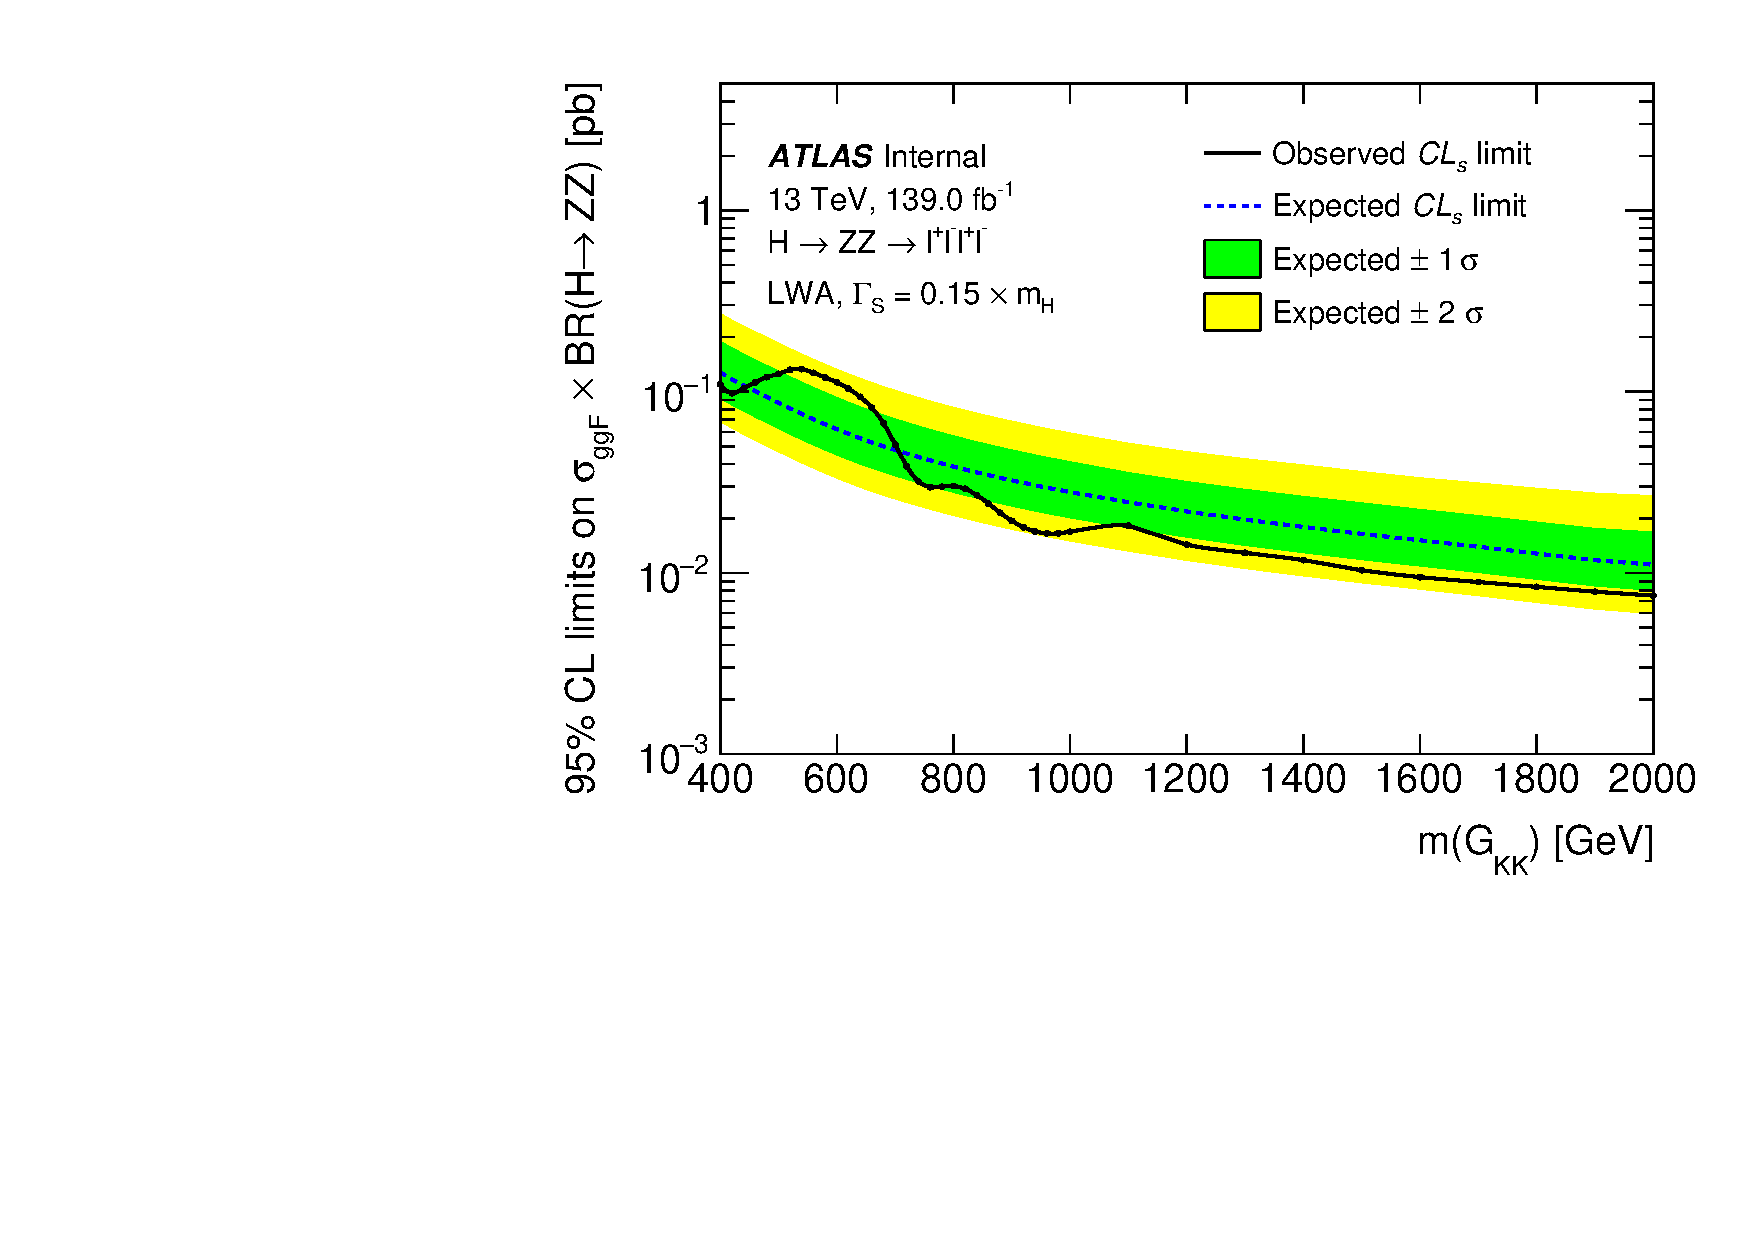
\includegraphics[width=0.48\textwidth]{figures/HMHZZ/results/Limits_LWA_withInt_15.pdf} \\
    \end{center}
    \caption{The upper limits at 95\% confidence level on $\sigma_{ggF} \times BR(H\rightarrow ZZ)$
    as a function of the heavy resonance mass $m_{H}$ for the ggF production mode with an intrinsic width of 1\% (top left), 5\% (top right), 10\% (bottom left) and 15\% (bottom right) for both the case where interference with Standard Model processes is considered.
    The green and yellow bands represent the $\pm 1~\sigma$ and $\pm 2~\sigma$ uncertainties in the expected limits.
  }
    \label{fig:LWAlimits_ggF_201518_withInt}
\end{figure}

\subsubsection{Spin-2 RS Graviton resonance}

The observed and expected 95\% upper limit on the cross section times branching ratio for RS Graviton (RSG) scenarios is shown in figure~\ref{fig:RSGlimits_ggF_201518}.
Same as LWA case, for RSG interpretation, only 4$e$, 4$\mu$ and 2$e$2$\mu$ channel of ggF production are used.
On top of the results in this analysis, a predicted cross section as function of mass provided by theorist is also shown.
Comparing with the observed result provided by $ZZ \rightarrow \llll$ decay, this spin-2 graviton is excluded up to a mass of around 1500~\gev.

\begin{figure}[h]
    \begin{center}
    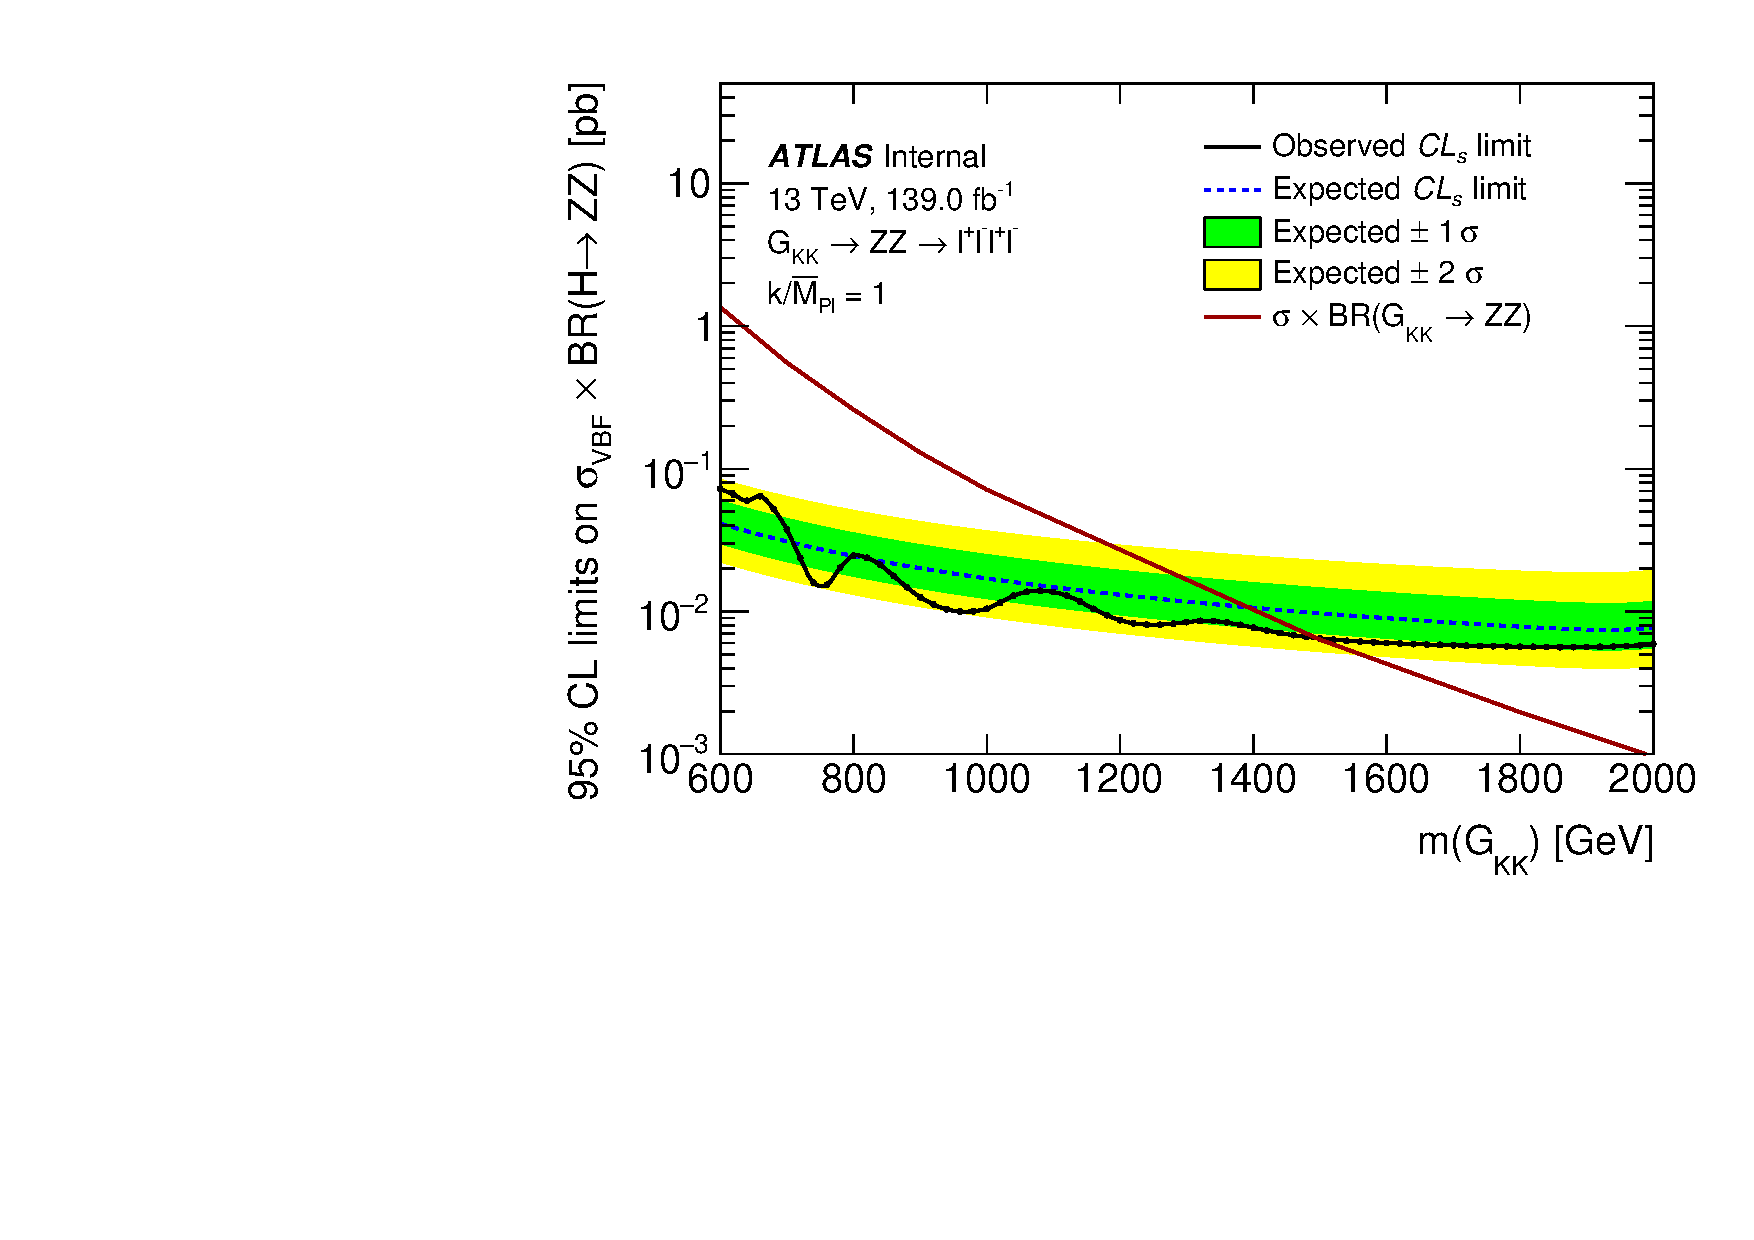
\includegraphics[width=0.48\textwidth]{figures/HMHZZ/results/Limits_RSG.pdf}
    \end{center}
    \caption{The upper limits at 95\% confidence level on $\sigma_{ggF} \times BR(G_{KK}\rightarrow ZZ)$
    as a function of the heavy resonance mass $m(G_{KK})$ for the ggF production mode in RS Graviton model.
    The green and yellow bands represent the $\pm 1~\sigma$ and $\pm 2~\sigma$ uncertainties in the expected limits.
  }
    \label{fig:RSGlimits_ggF_201518}
\end{figure}

\subsubsection{Comparison between different models}

As a summary, figure~\ref{fig:models_limits} shows the comparison of expected and observed 95\% CL upper limits between different models described above.

\begin{figure}[h]
    \centering
    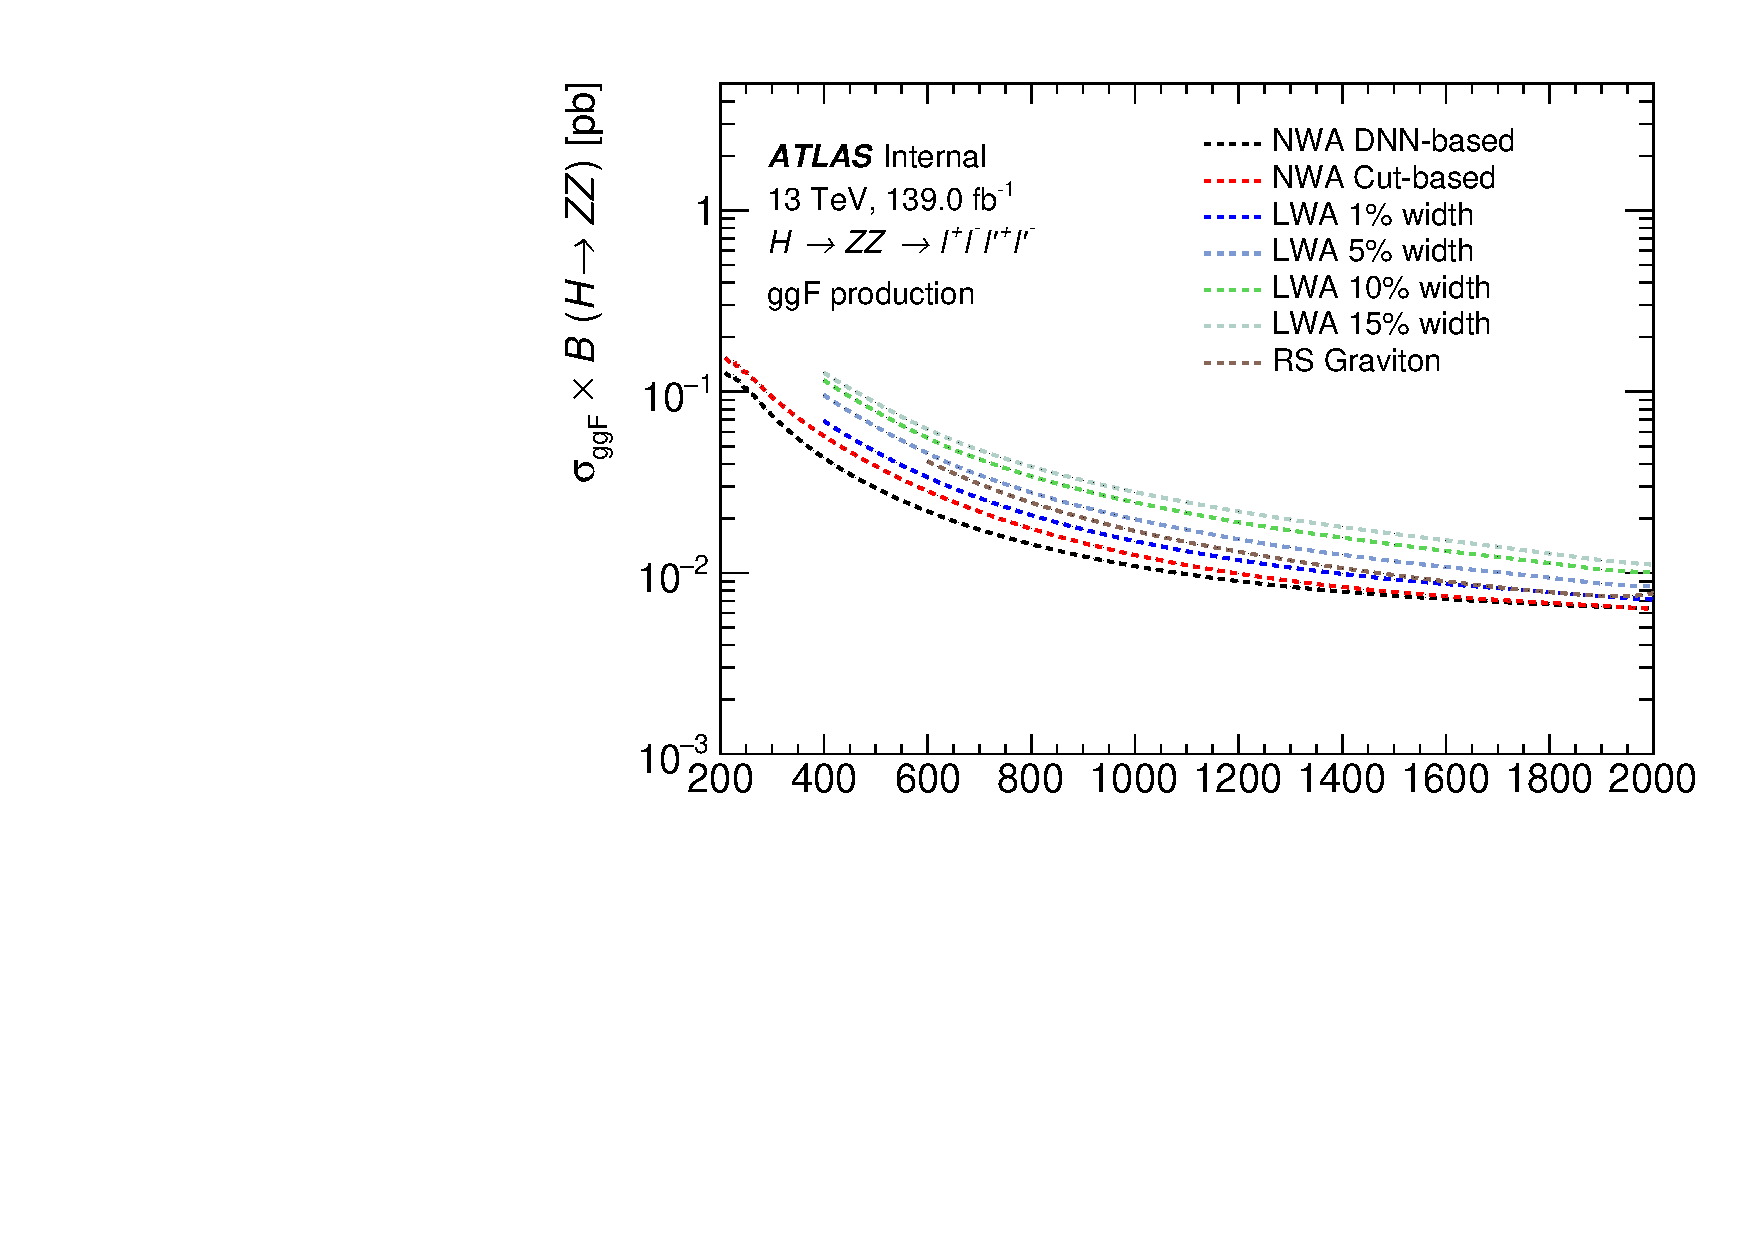
\includegraphics[width=0.48\textwidth]{figures/HMHZZ/results/4l_compareAll_exp.pdf}
    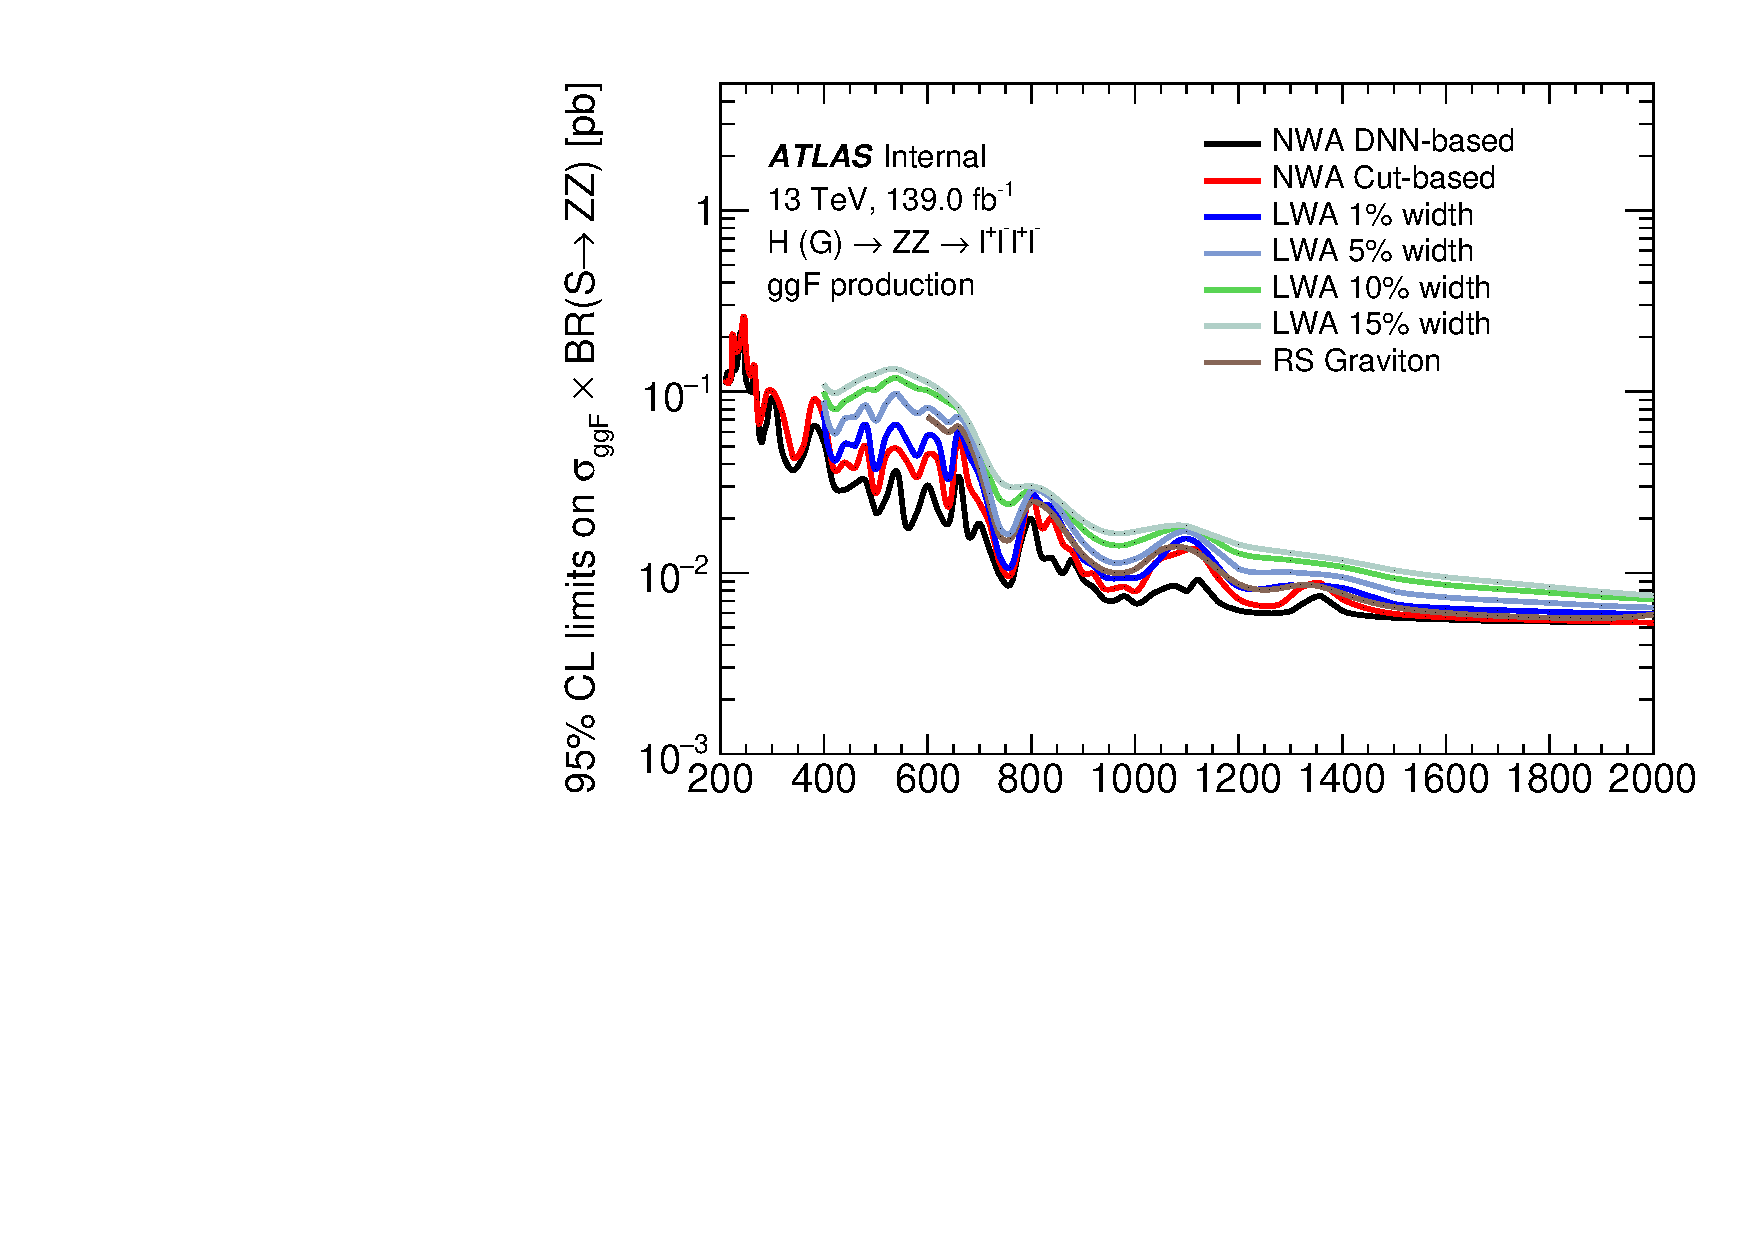
\includegraphics[width=0.48\textwidth]{figures/HMHZZ/results/4l_compareAll_obs.pdf}
    \caption{The expected (left) and observed (right) upper limits at 95\% confidence level on $\sigma \times BR(S\to ZZ)$ for ggF production mode at different assumptions. }
    \label{fig:models_limits}
\end{figure}
